% options:
% thesis=B bachelor's thesis
% thesis=M master's thesis
% czech thesis in Czech language
% english thesis in English language
% hidelinks remove colour boxes around hyperlinks

\documentclass[thesis=M,english]{FITthesis}[2018/10/20]

% \usepackage[utf8]{inputenc} % LaTeX source encoded as UTF-8
% \usepackage[latin2]{inputenc} % LaTeX source encoded as ISO-8859-2
% \usepackage[cp1250]{inputenc} % LaTeX source encoded as Windows-1250

\usepackage{graphicx} %graphics files inclusion
\usepackage{listings}
% \usepackage{subfig} %subfigures
% \usepackage{amsmath} %advanced maths
% \usepackage{amssymb} %additional math symbols

\newcommand{\code}[1]{\texttt{#1}}
\usepackage{float}

\setcounter{tocdepth}{3}% Include \substryAubsection in ToC

\usepackage{svg}

\usepackage{dirtree} %directory tree visualisation

% % list of acronyms
% \usepackage[acronym,nonumberlist,toc,numberedsection=autolabel]{glossaries}
% \iflanguage{czech}{\renewcommand*{\acronymname}{Seznam pou{\v z}it{\' y}ch zkratek}}{}
% \makeglossaries

% % % % % % % % % % % % % % % % % % % % % % % % % % % % % %
% EDIT THIS
% % % % % % % % % % % % % % % % % % % % % % % % % % % % % %

\department{Department of System Programming}
\title{GNU-R Debugger Bytecode Support}
\authorGN{Ale{\v s}} %author's given name/names
\authorFN{Saska} %author's surname
\author{Ale{\v s} Saska} %author's name without academic degrees
\authorWithDegrees{Bc. Ale{\v s} Saska} %author's name with academic degrees
\supervisor{Ing. Petr M{\' a}j}
\acknowledgements{Thanks to my adviser Petr M{\' a}j for help with reviewing thesis, Tom{\' a}{\v s} Kalibera for useful help with the GNU-R code and functionality, my father for assisting with the submission of this work, and big thanks to my girlfriend for psychological support and all the tea required to make this work happen.}
\abstractEN{This thesis is about analysis and implementation of the advanced bytecode disassembler tool for GNU-R language. The implemented tool is returning the information in a human readable, compact format for passed function. This second feature was reused in the second part of the thesis which is about native support for bytecode debugger. The current debugging options for the bytecode in GNU-R are insufficient because of implementing through AST call. The debugging capabilities of the languare are improved in this thesis by implementing native support for debugging bytecode. Presented implementation shows all internal information of the bytecode evaluator status. The solution written in this thesis is focusing on making any negative impact to the overall performance of the language which has been successfully tested and proven with testing.}
\abstractCS{Tato pr{\' a}ce se zabývá analýzou a implementací pokročilého bytecode debuggeru pro jazyk GNU-R. Implementovaný systém vypisuje informace v čitelné a uživatelem srozumitelné podobě pro každou instrukci zadané funkce. Druhá část práce se zabývá

 V n{\v e}kolika v{\v e}t{\' a}ch shr{\v n}te obsah a p{\v r}{\' i}nos t{\' e}to pr{\' a}ce v {\v c}esk{\' e}m jazyce.}
\placeForDeclarationOfAuthenticity{Prague}
\keywordsCS{Replace with comma-separated list of keywords in Czech.}
\keywordsEN{computer language,R,GNU-R,bytecode,disassembler,debugger}
\declarationOfAuthenticityOption{1} %select as appropriate, according to the desired license (integer 1-6)
% \website{http://site.example/thesis} %optional thesis URL



\begin{document}

%\captionsetup{justification=centering}

% \newacronym{CVUT}{{\v C}VUT}{{\v C}esk{\' e} vysok{\' e} u{\v c}en{\' i} technick{\' e} v Praze}
% \newacronym{FIT}{FIT}{Fakulta informa{\v c}n{\' i}ch technologi{\' i}}

\setsecnumdepth{part}
\chapter{Introduction}\label{introduction}

\section{Motivation and objectives}\label{motivation-and-objectives}

Almost everyone who has been trying to write computer program has made some logical mistakes in them. To help to solve them, we usually run program \textbf{step-by-step} with debugging tools with some debugger. The \mbox{\textbf{GNU-R}} which is one of the most widely used scientific languages across the whole world also has its implementation for debugging code.

GNU-R language is dynamically typed interpreted language which usually means that it needs \textbf{Virtual Machine} to interpret. There are more ways to represent and implement its evaluation. The first one \textbf{Abstract Syntax Tree}~(see~\ref{AST}) evaluation is the simplest one. To make speedup of its internal evaluation, there has been introduced the \textbf{Bytecode}~(see~\ref{BC}) compiler and interpreter into \mbox{GNU-R} in 1998.

While the abstract syntax evaluator is the slowest of the two analyzers it already contains the debugging features GNU-R implemented. However, it was previously difficult to analyze and debug the other analyzer, bytecode. The only method provided to analyze the bytecode is very basic disassembler showing the data in human unfriendly way. It means that there is currently no support for real-time debugging of GNU-R bytecode evaluation. Instead of it there is implemented switching into the AST interpreter once user requests the debugging features. The whole lack of the native bytecode debugger is causing potential issues because the code used for bytecode can be slightly different than the code used while not-debugging~(AST one) even if it produces the same result. Eventually, this can also cause an issue when there is an error inside AST or BC interpreter core. This can result in confusing and very hard to solve issue.

The work done in this thesis is solving the insufficient \textbf{bytecode disassembler} by replacing it with a \textbf{new easy-to-use and human-friendly one}. The another implemented feature is \textbf{advanced and user-friendly native support for bytecode debugger} which is significantly improving the options for analysis and debugging any program code running on the bytecode engine of the language. This implementation was written with the focus on having any performance slowdown of the bytecode engine which was proven in the performance testing part on the ending of the work. On top of this, there was implemented the feature containing \textbf{breakpoint instruction} which is used for the \textbf{simulation of the conditional breakpoints}.

All the implemented features were successfully tested. The disassembler \code{bctools} package has written automated tests and there was concluded an performance testing of the GNU-R engine. 

This thesis is organized as follows: Section~\ref{introduction} is the introduction into problems of dynamic languages evaluation. Section~\ref{analysis-of-disassembler} contains the analysis of possible solutions how to implement the bytecode disassembler and the debugger. Section~\ref{realization} is describing design of current implementation. Section~\ref{testing-and-future-work} describes what type of testing has been done on the work. Section~\ref{testing-and-future-work} proposing work for the future improvements of the work followed by thesis summarization in conclusion.

%\section{Problem statements}

%There are two main types of programming languages. Dynamic typed and static typed ones.
%Static such as \textbf{C} / \textbf{C++} / \textbf{FORTRAN} languages has strictly defined types and are usually more machine inspired/focused. Dynamic ones usually do not have strict type inference so they allow the user~(programmer) more freedom. As trade-off they usually needs Virtual Machine~(\textbf{VM}, see~\ref{VM}) to runs efficiently which cause possible performance slowdown. \textbf{GNU R} language was primarily developed for the scientists so user-friendliness and no need to necessary care about data types was one of the decision to make the language dynamic typed.

%TODO: add more of some good shit

\setsecnumdepth{all}
%\chapter{State-of-the-art}

\chapter{Analysis and design}

\section{GNU R from user perspective}\label{R-UI}

\subsection{Basis usage~(main commands and REPL loop)}\label{REPL}

The main \textbf{GNU R} language is written as the console application evaluating the infinite \textbf{REPL} - Read Eval Print Loop. As the abbreviation says, it is evaluating the expressions right as is entered by the user~(of the \code{R} program) to the program standard input~(\code{stdin}). Alongside of this, there is also the \code{Rscript} command in the package which supports running the program from the input file. However, it is internally implemented just as wrapper piping the file content into the \code{R} command.

\subsection{GNU R package system}\label{R-Packages}

The \textbf{GNU-R} has integrated package subsystem \textbf{CRAN} with plenty of inbuilt packages. These packages are intended to be the easy way for developers~(R users) how to make a user-friendly extension for other people. The bytecode compiler is written in the GNU-R in the separate package named \code{compiler}. This package comes already pre-installed so users don't need to manipulate with it as with the other user-installed libraries. However, the bytecode disassembler in this thesis is written as the separate package named \code{bctools} because it is better to keep the language core minimal and the disassembly tool can be implemented as a plugin into the language.

Because we would be creating our package we need to be able to manipulate and work with it. These are few basic commands to work with packages:

\begin{itemize}
	\item \code{R CMD INSTALL $<$pkgs$>$ } - install specified packages
	\item \code{R CMD build $<$pkgname$>$} - build the package
	\item \code{R CMD check $<$pkgname$>$} - check package~(check requirements, run tests, etc.)
\end{itemize}



\subsection{GNU R class system}\label{R-Classes}

Classes are way how to in Object-oriented Programming (OOP) group functionality of one meaning. For example instead of the two functions \code{drawButton} and \code{pressButton} we can have the two methods \code{draw} and \code{press} belonging to the object \code{button}. The GNU-R is dynamic language it is variable can be any type. It means that once we'd call method of class (function on the variable), the language engine has to look up the specific code for the class which would be then evaluated. This functionality also is used in the printing of the values or objects via the \code{print} method which we can use for the disassembler. The user would then be able to print out the disassembly in the same way as he is used with other data types. The \code{print} method is also dispatched by default in the REPL loop in printing phase.

According to the Hadley Wickham's article about GNU-R	 has 4 possible class systems - \textbf{\code{S3}}, \textbf{\code{S4}}, \textbf{Reference classes} and \textbf{Base classes}~(internally used). It means that the \textbf{R} class system is not strictly defined as in languages like Java, C++, \textbf{Python}, etc. The whole system provides the end user to more flexibility, but on the other hand, it can be a little bit more confusing for the programmers who are used to conventional programming languages.

The system used in the print method is \code{S3}. It implements a style of OO programming called generic-function OO. This is different from most programming languages, like Java, C++, and C{\#}, which implement message-passing OO. With message-passing, messages~(methods) are sent to objects and the object determines which function to call. Typically, this object has a special appearance in the method call, usually appearing before the name of the method/message: e.g., \code{canvas.drawRect("blue")}. S3 is different. While computations are still carried out via methods, a special type of function called a generic function decides which method to call, e.g., \code{drawRect(canvas, "blue")}. S3 is a very casual system. It has no formal definition of classes.

%\item \textbf{S4} works similarly to S3, but is more formal. There are two major differences to S3. S4 has formal class definitions, which describe the representation and inheritance for each class, and has special helper functions for defining generics and methods. S4 also has multiple dispatch, which means that generic functions can pick methods based on the class of any number of arguments, not just one.

%\item \textbf{Reference classes}, called RC for short, are quite different from S3 and S4. RC implements message-passing OO, so methods belong to classes, not functions. {\$} is used to separate objects and methods, so method calls look like \textit{canvas{\$}drawRect("blue")}. RC objects are also mutable: they don't use R's usual copy-on-modify semantics, but are modified in place. This makes them harder to reason about, but allows them to solve problems that are difficult to solve with S3 or S4.


%There's also one other system that's not quite OO, but it's important to mention here:


%\item \textbf{base types}, the internal C-level types that underlie the other OO systems. Base types are mostly manipulated using C code, but they're important to know about because they provide the building blocks for the other OO systems.
%\end{itemize}


\section{GNU R internal structure}\label{R-internal-structure}

The core GNU-R VM core is written in C language with the broad number of supported platforms~(Windows/MAC/Linux...) and computer architectures~(ARM/x86/x64...). The multi-compiler support also means that there could be the difference in supported features which would need conditional checks for supporting this feature in the compiler code. One of the examples is support for the Computed GOTO~\ref{Computed-GOTO}.

\subsection{Implementation of the core features of the language in R itself}

The GNU-R has internally written the loading mechanism in the way that the \code{base} package is loaded first and then all of the packages contained in list \code{getOption("defaultPackages")} are loaded into the global environment. This mechanism allows that just the core features and language constructs are written in performance-optimized \code{C}, and the rest can be written inside R language itself. It means that inside these packages there is substantial amount of functionality for the whole language. The \code{compiler} package is little different than the other packages because it needs to be loaded due to internal bytecode compiler usage~(see JIT chapter~\ref{JIT}). However, it's loading mechanism is different because it is hardcoded in the code. It is hardcoded in \code{loadCompilerNamespace}~(in the \textit{src/main/eval.c} file) to be independent on the whole code.

%TODO: clean it up

\subsection{Calling internal C functions from R}

%TODO: REWRITE IT

\textbf{C code} compiled into R at build time can be called directly in what are termed primitives or via the \code{.Internal} interface, which is very similar to the \code{.External} interface except in syntax. More precisely, R keeps a table of function names and corresponding C functions to call, which by convention all start with \code{do{\_}} and return a \code{SEXP}. This table (\code{R{\_}FunTab} sitting in file \textit{src/main/names.c}) also specifies how many arguments to a function are required or allowed, whether or not the arguments are to be evaluated before calling, and whether the function is internal in the sense that it must be accessed via the \textbf{.Internal} interface, or directly accessible in which case it is printed in \textbf{R} as \textbf{.Primitive}.

\section{Computer Program Compiler Structure}

%\subsection{Internal structure}\label{Compiler-internal-structure}

%To make compilers structure internally more organized most of the compilers or \textbf{VM}s are divided into separate passes.

%The common basic ones are:
%\begin{itemize}
%	\item Frontend - parsing source code into %\textbf{IR} or \textbf{AST}~(see chapter~%\ref{AST} )
%	\item Optimizer - optimizing \textbf{IR} or \textbf{AST}~(can be left out)
%	\item Backend - generating machine code or running \textbf{VM}~(see chapter~\ref{VM})
%\end{itemize}
%Each step can be also divided into more steps (for example frontend consists usually of lexer and parser).

%As long as the \textbf{GNU R} is dynamic language it is build over the internal Virtual Machine. It does an on-demand parsing of the source code which directly evaluates.

%The optimization problem is very difficult inside the \textbf{GNU R}. One of its' example why this is not possible is extreme dynamism of the language. For example you can:
%\begin{itemize}
%	\item Change the body, arguments, and %environment of functions.
%	\item Change the S4 methods for a generic.
%	\item Add new fields to an S3 object, or %even change its class.
%	\item Modify objects outside of the local %environment with <<-.
%\end{itemize}

%Basically the \textbf{GNU R} is monolithic structure built in over the Virtual Machine. This design is not ideal but it came up from to historic reasons.

\subsection{Virtual Machine}\label{VM}

Static languages compilers usually use directly the computer operating system as the running environment. However, the GNU-R is the dynamically typed computer language with the internal Virtual Machine~(VM) providing the \textbf{running environment}.
It is simulating the environment by executing code, managing memory, and providing communication layer with the underlying computer and its external devices ( accessing the filesystem, network communication, etc. ). The nature of all being simulated usually results in performance slowdown, but on the other hand, there is s significant safety advantage of isolation which results of the code being much safer.

There are more types of virtual machines. The most common ones are stack machines followed by the register-based machines.

The \textbf{register-based} ones simulate register processors (such as \textbf{x86} architecture Intel or \textbf{ARM} ones) with instructions which are capable of working with more registers. The bigger number of registers implicates more sophisticated instructions because they needs to contain information about what registers should be accessed (for example Android \textbf{Dalvik VM} \code{add-int} instruction has 3 parameters - Destination parameter, the first source register, and second source register ). The more information which the instruction needs to contain results in longer instruction sizes and more expensive instruction decoding which both negatively impacts execution speed. However, they can profit from the nature of the register-based hardware of the most common processor architectures~(ARM, x86, etc.) so they should get better evaluation performance.

The \textbf{stack-based} ones, on the other hand, are simpler ones because every instruction arguments lie on the top of the stack in the specified order (for example ADD instruction removes two topmost arguments from the stack, make the addition, and push back the result to the stack). The simplicity of instruction coding implies easier instructions and also easier implementation of both compiler and evaluator code. This type is one of the most common and also the GNU R Bytecode engine one of its representative.

The examples of virtual machines are
\begin{itemize}
	\item JVM - Java VM
	\item Python
	\item GNU R
	\item Dalvik VM - Android VM ( the only register one based in this list )
	\item JavaScript V8
	\item Chakra ( JavaScript inside MS Edge browser)
\end{itemize}

\subsubsection{Internal parts of the VM}\label{internal-parts-of-vm}

\textbf{GNU R} virtual machine is stack based one. Due to simplicity it consists of these parts:
\begin{itemize}
	\item \textbf{Parser} (mainly in src/main/gram.y which generates src/main/gram.c)
	\item \textbf{Memory management} ( mainly in src/main/memory.c )
	\item \textbf{AST evaluator} ( eval function inside src/main/eval.c )
	\item \textbf{Bytecode Compiler} ( inside R package Compiler )
	\item \textbf{Bytecode evaluator} ( bcEval function inside src/main/eval.c )
	\item \textbf{Runtime environment}
\end{itemize}

\subsection{GNU R memory types and memory management}\label{memory-management}

Each memory node is represented as \code{SEXP} type. It contains internal representations such as code definition ( \code{LANGSXP}, \code{BCOSESXP}, \code{WEAKREFSXP}, promises, etc. ) and also regular memory types (such as logical vectors, integer vectors, strings vectors, etc.). GNU-R is a vector language, so every value is internally represented as a vector (e.g., integer 3 is represented and boxed as \code{INTSXP} vector of size 1 containing value 3).

Types of memory nodes are

\begin{itemize}
	\item \textbf{NILSXP} nil = NULL
	\item \textbf{SYMSXP}	     symbols
	\item \textbf{LISTSXP}	     lists of dotted pairs
	\item \textbf{CLOSXP}	     closures
	\item \textbf{ENVSXP}	     environments
	\item \textbf{PROMSXP}	     promises: [un]evaluated closure arguments
	\item \textbf{LANGSXP}	     language constructs (special lists)
	\item \textbf{SPECIALSXP}   	special forms
	\item \textbf{BUILTINSXP}   	builtin non-special forms
	\item \textbf{CHARSXP}	     "scalar" string type (internal only)
	\item \textbf{LGLSXP}	    logical vectors
% 11 and 12 were factors and ordered factors in the 1990s
	\item \textbf{INTSXP}	    integer vectors
	\item \textbf{REALSXP}	    real variables
	\item \textbf{CPLXSXP}	    complex variables
	\item \textbf{STRSXP}	    string vectors
	\item \textbf{DOTSXP}	    dot-dot-dot object
	\item \textbf{ANYSXP}	    make "any" args work.
%			     Used in specifying types for symbol
%			     registration to mean anything is okay
	\item \textbf{VECSXP}	    generic vectors
	\item \textbf{EXPRSXP}	    expressions vectors
	\item \textbf{BCODESXP}    byte code
	\item \textbf{EXTPTRSXP}   external pointer
	\item \textbf{WEAKREFSXP}  weak reference
	\item \textbf{RAWSXP}      raw bytes
	\item \textbf{S4SXP}       S4, non-vector
% used for detecting PROTECT issues in memory.c
	\item \textbf{NEWSXP}      fresh node created in new page
	\item \textbf{FREESXP}     node released by GC

	\item \textbf{FUNSXP}      Closure or Builtin or Special
\end{itemize}

These types are holding values which can be printed in the disassembler function~\ref{implementation-of-disassembler} and also inside the stack printer~\ref{printing-stack-values} in this thesis.

\subsection{GNU R garbage collector}\label{GC}

The memory management in dynamic languages is maintained by  \textbf{Garbage Collector}. It releases allocated memory once it is no longer used by program. GNU R implementation of memory management lies inside \textit{src/main/memory.c}. It implements a non-moving generational garbage collector with two or three generations. Memory is allocated by \code{R{\_}alloc} and is maintained in a stack. There is also protection stack managed by \code{PROTECT}~(and \code{UNPROTECT}) functions which is used inside C code for internal purposes~(widely used in~\ref{implementation-of-debugger}). It allows to push locally allocated variables into it so they are reachable by the garbage collector and would not get removed during a garbage collection run~(memory cleanup).

\subsection{Computed GOTO}\label{Computed-GOTO}

The Computed GOTO technique is used in the VM for code \textbf{evaluation speedup}. Also, the GNU-R VM has its internal support for this feature~(managed by macro \code{THREADED{\_}CODE}). Because the DEBUG instruction is internally dispatching an old previous instruction after execution of debug features there was a need to understand the whole bytecode instruction jumping.

\textbf{GNU R} has the support of threaded code~(implemented by the \textbf{computed GOTO} technique) although there is still support for non-GCC compilers~(and compilers which does not support this feature) - see~\ref{VM}. Enabling or disabling of this feature is managed by (\code{THREADED{\_}CODE} \code{define} preprocessor command.

The all of the while loop and switch cases are in the GNU-R code then defined with macros~(\code{INITIALIZE{\_}MACHINE}, \code{BEGIN{\_}MACHINE}, \code{OP}, \code{NEXT} and \code{LASTOP}). They are conditionally defined to either be compiled for supporting Computed GOTO~\ref{computed-goto-used} or not~\ref{computed-goto-used}~(according to the \code{THREADED{\_}CODE} flag).

\subsubsection{Computed GOTO not used - Switch dispatch}\label{computed-goto-not-used}

The internal representation of the traditional implementation of the BC evaluator acts like big loop going through all function instructions. It causes that in each loop step there has to be branching of program flow according to instruction~(\code{if} command). In the traditional way, this is done as the switch-case where case values are the instruction codes. Example of this approach:

\begin{figure}[!htb]
\begin{lstlisting}
while(1){
  switch(*opcode++){
    case POP:	//POP=1
      ... do instruction POP ....
      break;
    case GETVAR:	//GETVAR=2
      ... do instruction GETVAR ....
      break;
    case ADD:	//GETVAR=3
      ... do instruction ADD ....
      break;
  }
}
\end{lstlisting}
\caption{\label{fig:goto-not-used} Example of the VM with switch dispatch architecture.}
\end{figure}

\subsubsection{Computed GOTO used - threaded code}\label{computed-goto-used}

The \code{switch} statement should be implemented very efficiently by C compilers - the condition serves as an offset into a lookup table that says where to jump next which means that it is evaluated for every bytecode instruction. However, it turns out that there's a popular GCC extension that allows the compiler to generate even \textbf{faster code}. The main idea behind this is to store the address of the label into the value of a variable which allows the dynamic lookup of the next value.

%Example of computed-goto code:
\begin{figure}[!htb]
\begin{lstlisting}
/* The indices of labels in the dispatch_table
 * are the relevant opcodes
 */
static void* dispatch_table[] = {
        &&do_halt, &&do_inc, &&do_dec, &&do_mul2,
        &&do_div2, &&do_add7, &&do_neg};
#define DISPATCH() goto *dispatch_table[code[pc++]]

int pc = 0;
int val = initval;

DISPATCH();
while (1) {
    do_halt:
        return val;
    do_inc:
        val++;
        DISPATCH();
    do_dec:
        val--;
        DISPATCH();
    do_mul2:
        val *= 2;
        DISPATCH();
}
\end{lstlisting}
\caption{\label{fig:goto-used-table} Example of the VM with computed goto architecture through dispatch table.}
\end{figure}

In the GNU-R implementation of bytecode interpreter, there is performance optimization called \textbf{direct threaded code}  associated with dispatch table and the \textbf{computed GOTO}. In process of loading bytecode into the VM internal structure~(done by \code{R{\_}bcDecode} and \code{R{\_}bcEncode} functions inside \textit{src/main/eval.c}) there is translation between instruction codes~(integer codes) and the current location of jump labels inside \code{bcEval} - see \textit{computed goto}~\ref{AST}(\code{void*} type). The nature of the operating system loader would cause that this position can~(and usually is) changed every time the program is started~(R VM is loaded into memory by a operating system) - so value has to be computed every time again. This allows BC interpreter to jump directly at the position which is stored inside the code array. It would cause saving one array lookup every step of BC interpreter compared to the classic interpreter~(implemented for example inside \textbf{CPython} VM).

\subsection{Abstract Syntax Tree}\label{AST}

To be able to internally interpret the syntax of every language the code is first parsed into abstract syntax tree~(\textbf{AST}, see the example in fig.~\ref{fig:ast-while}). Tree in the GNU-R contains nodes of LANGSXP type with references to the symbol table~(pointers to the function). These references are represented as an pointers to functions which have implemented the evaluation of the code. This tree is then traversed and evaluated inside \code{eval} function~(which lies in file \textit{src/main/eval.c}). The evaluator also has built-in support for debugging which is done internally by the checking of the \code{RDEBUG} flag of the current executed environment. The flag is checked every evaluator step which creates performance overhead even though the debug mode is not active. However this checking overhead is usually minimized by branch prediction feature of current CPUs. 

The current AST evaluator debugging implementation was in this thesis used as an inspiration for the functionality of the newly implemented features~\ref{implementation-of-debugger}. The other thing inspired by the this debugger is the user-output in case the bytecode debugger is in the non-verbose mode. In that case the bytecode debugger is simulating the command-line behavior of the AST - see section~\ref{short-compact-way-of-status-printing}.

%TODO: reference to the branch prediction

\begin{figure}[hH!]\centering
	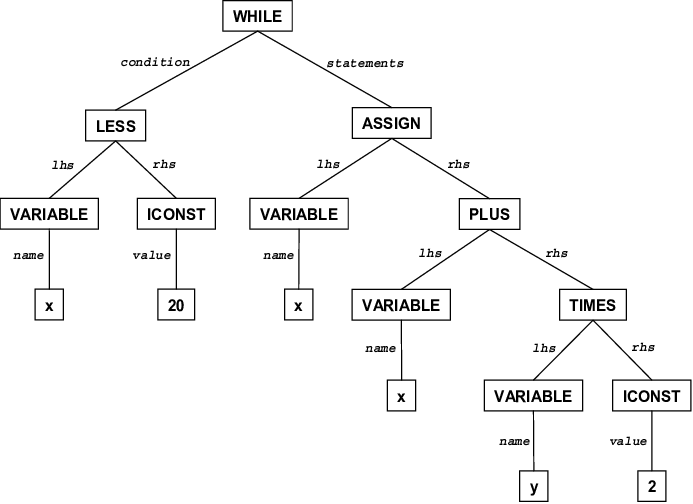
\includegraphics{Abstract-syntax-tree-of-the-while-loop}
	\caption{While loop example}\label{fig:ast-while}
\end{figure}

\subsection{Bytecode}\label{BC}

Another option how to represent the source code to evaluate is the \textbf{bytecode}. It has an array of transferable instruction codes and constants designed for easy evaluation. The name bytecode stems from the the instruction set that have one byte operation code. Structure contains the instruction code which follows parameters (depending on how many / if parameter given instruction have ). This thesis content is about an implementation of support for the bytecode evaluator of an GNU-R language.

\subsection{Just in Time compilation}\label{JIT}

In order to speed-up evaluation of inside \textbf{VM}, there have been developed various techniques of the \textbf{performance optimization}. One of them is Just in Time~(JIT) compilation of code. The underlying idea is to internally translate code into some more efficient representation ( from \textbf{AST} to either \textbf{Bytecode} or to the native machine code ). However, this transformation (compilation) is usually pretty expensive so it is called once the execution of a specified piece of code reached some limit.
GNU-R has the basic internal support of \textbf{JIT}. Implementation lies inside \code{src/main/eval.c} mainly in functions \code{R{\_}CheckJIT} and \code{R{\_}cmpfun} ). It is executing the \code{Compiler::tryCmpfun} to compile function \textbf{AST} into \textbf{bytecode}. According to the posts from running code with ByteCode, the JIT enables speedup up to 10 times~(theoretically up to 25 times but these cases are very rare).
This means that the bytecode engine of GNU-R code can be used even without a user knowing it~(explicitly calling compilation) which would make work for the bytecode debugger in our thesis very important. The second important thing is that both interpreters~(AST and BC one) can be run together therefore there has to be a need to clearly decide which is currently in use~(this feature is implemented in chapter~\ref{bytecode-interpreter-internal-status}).

%TODO: JIT speedup by citation

%As mentioned before, the compilation can take significant amount time, so it makes sense for the virtual machine to compile just the most used parts of code~(if the every function would be compiled, it would have even cause the slowdown). The \textbf{GNU R} has for this more strategies:

%\begin{itemize}
%  \item \textit{NO{\_}CACHE}
%
%      functions are compiled 1st time seen
%
%      \hspace*{6mm} code is never cached
%
%  \item \textit{NO{\_}SCORE}
%
%      functions are compiled 1st time seen,
%
%      \hspace*{6mm} code is cached,
%
%      in case of conflict function may be marked \textit{NOJIT}
%
%  \item \textit{ALL{\_}SMALL{\_}MAYBE}
%
%      functions with small score are compiled 2nd time seen,
%
%      function with high score are compiled,
%
%      \hspace*{6mm} 1st time seen if top-level, 2nd time seen %otherwise
%
%  \item \textit{TOP{\_}SMALL{\_}MAYBE}
%
%      functions with small score compiled,
%
%      \hspace*{6mm} 2nd time seen if top-level, never otherwise
%
%      functions with high score compiled
%
%      \hspace*{6mm} time seen if top-level, 2nd time seen otherwise
%\end{itemize}

\subsection{Computer language promises}\label{computer-promises}

GNU-R computer language is heavily dependent on the promise pattern. As its name says this pattern represents a promise into the future that some code would be evaluated~(instead of running it immediately). For example instead direct call (see figure~\ref{fig:reading-csv-without-promise}) you can manually force GNU-R to wrap the function evaluation in the promise via the \code{future} function (see figure~\ref{fig:reading-csv-with-promise}).

\begin{figure}[!h]
\begin{lstlisting}
#fires immediatelly the read function
value <- read.csv(... some datafile ...)

#just prints the value
print(value)
\end{lstlisting}
\caption{\label{fig:reading-csv-without-promise} GNU R - reading an data from csv table}
\end{figure}

\begin{figure}[!h]
\begin{lstlisting}
#create just an promise containing the read function call
value <- future(read.csv(... some datafile ...))

#evaluates the promise (do the read.csv function)
#  on the background
#  and finally printing out the result
print(value)
\end{lstlisting}
\caption{\label{fig:reading-csv-with-promise} GNU R - reading an data from csv table wrapped in promise}
\end{figure}

This shown approach is manual and pretty straightforward for the user to understand. However, the GNU-R has promise based lazy evaluation of arguments. Every argument in the function is the promise and instead of evaluating it before the function call~(like in other old-fashioned languages like \code{C} or \code{Java}), the argument is evaluated inside the function code once it is accessed~(see the figure~\ref{gnu-r-promise-arguments}). It causes that the GNU-R is internally heavy dependent on the promises even it is not obvious for the normal user at the first sight. The promises and printing of their content was done in this thesis in the stack printer~\ref{implementation-of-stack-printer}.

\begin{figure}[!h]
\begin{lstlisting}
getB <- function(){
	print("getB")
	5
}

calc <- function(a,b){
	print("calc enter")
	ret <- a*2
	print("accessB")
	ret <- b*10
	print("calc exit")
}
calc(2,getB())

#will produce output:
# [1] "calc enter"
# [1] "accessB"
# [1] "getB"
# [1] "calc exit"
\end{lstlisting}
\caption{\label{fig:gnu-r-promise-arguments} GNU R - example of promise based arguments evaluation}
\end{figure}


\begin{lstlisting}

\end{lstlisting}


\section{GNU R Bytecode}

GNU-R has the internal support of the BC which consists of \code{compiler} package for compiling to the bytecode. The language bytecode is interpreter by function \code{bcEval}~(inside \textit{src/main/eval.c}). The BC compiler can be used explicitly by calling certain functions to carry out compilations or implicitly by enabling compilation to occur automatically at certain points.

\begin{itemize}
  \item \textbf{Explicit compilation} - primary functions are: \code{compile}, \code{cmpfun}, \code{cmpfile}
  \item \textbf{Implicit compilation} - can be used to compile packages as they are installed or for JIT compilation of functions or expressions.

For now, the compilation of packages is enabled by calling \code{compilePKGS} with argument \code{TRUE} or by starting R with the environment variable \code{R{\_}COMPILE{\_}PKGS} set to the positive integer value.
\end{itemize}


\subsection{GNU R internal representation of bytecode}\label{R-internal-bc-representation}

The internal representation of bytecode is \code{SEXP} node of \code{BCODESXP} type. It is internally represented as a linked list~(CONS of cells) of two variables:
\begin{itemize}
	\item \textbf{Bytecode code}~(body) array which contains set bytecode instructions following its' parameters

		\hspace*{6mm} internally represented as first element~(\textit{CAR}) of the list

		\hspace*{6mm} accessed in the code through the \code{BCODE{\_}CODE} macro

		\hspace*{6mm} The array contains the representation of version number followed by the bytecode instructions

	\item \textbf{Constant pool} array

		\hspace*{6mm} internally represented as second element~(\textit{CDR}) of the linked list

		\hspace*{6mm} accessed in the code through the \code{BCODE{\_}CONSTS} macro

		\hspace*{6mm} contains the of the constant expressions~(which are referenced in the bytecode array)

\end{itemize}

\subsection{Expression and source references}\label{Exprref-and-srcref}

At the end of the constant pool array, there can be~(are optional) some additional information about the bytecode. This information is not used for the evaluation but are provided for specifying the original location of the compiled code. They are used in the disassembler tool~\ref{implementation-of-disassembler} and are used in the implemented feature which is doing jumping granularity restriction~\ref{debugger-jumping-granuality}. They can be of 2 types:

\begin{itemize}
	\item \textbf{Expression reference}

describing the expression representation of bytecode~(for example \textit{b+a+4})

	\item \textbf{Source reference}

describing the location in the source file~(for example \textit{main.R{\#}4})
\end{itemize}

The data structures in the end of the constant array can contain these class types:

\begin{itemize}
	\item \textbf{srcref}

Source reference representing the whole function~(it's beginning)

	\item \textbf{srcrefsIndex}

Array corresponding source references to code for each instruction~(length of the array is length of BC code array - see~\ref{R-internal-bc-representation})

	\item \textbf{expressionsIndex}

Array corresponding expression references~(expressions) to code for each instruction~(length of the array is the length of BC code array - see~\ref{R-internal-bc-representation})

\end{itemize}

\section{Current implementation of AST debugger}\label{AST-debugger}

AST evaluator of GNU-R is implemented as a recursive descent of the AST tree.
The current implementation of debugger inside  GNU-R language is made on top of the AST interpreter and it uses the \code{RDEBUG} flag of current evaluated to check if enable the debugging features. For user, there are written functions~(user interface) managing this functionality. They are:

\begin{itemize}
	\item \code{debug(fun, text = "", condition = NULL, signature = NULL)}

	\hspace*{6mm} enables debug features on the function~\code{fun}

	\item \code{debugonce(fun, text = "", condition = NULL, signature = NULL)}

	\hspace*{6mm} run debug features on the function~\code{fun} next time it is called

	\item \code{undebug(fun, signature = NULL)}

	\hspace*{6mm} disable debug features on the function~\code{fun}

	\item \code{isdebugged(fun, signature = NULL)}

	\hspace*{6mm} check whether the debugging features on the function~\code{fun} are enabled

	\item \code{debuggingState(on = NULL)}

	\hspace*{6mm} manages the debugging features by turning them off / on by managing R internal state

	\hspace*{6mm} returns boolean representing whether debugging is globally turned on. In the case that the \code{on} parameter is not NULL, the internal state is modified according to that parameter.

\end{itemize}

To keep the same debug functionality for functions running on top of the bytecode there is a fallback for switching back to the AST implementation. It implicates that for users the code behaves in the same way~(both BC and AST representation are producing equivalent output), but can cause issues when there are bugs in the internal engine~(either AST or BC evaluator). In that case, the code while debugging would be using the different code than while not-debugging. This can potentially cause confusing and hard to solve issues. 

There is currently also no way to debug BC internals~(stack content and showing the current evaluating instruction in the code) while running. This would be changed in this work by implementing an stack printer~\ref{implementation-of-stack-printer} and disassembler~\ref{implementation-of-disassembler}.

The GNU-R debugger internal implementation of interacting with the user is made by calling the \code{browse()} function which is running the environment browser. Its purpose is to wait for user input. Once the user types expression, it evaluates the typed expression. Its internal representation is reusing the function shared with main REPL loop~(mainly functions \code{Rf{\_}ReplIteration} and \code{ParseBrowser} inside \textit{src/main/main.c}) for support user input~(parsing and evaluating).

The \code{browse()} function also has support for the commands managing the debug mode. They are:
\begin{itemize}
\item \code{c} - exit the browser and continue execution at the next statement.
\item \code{cont} - a synonym for c.
\item \code{f} - finish execution of the current loop or function
\item \code{help} - print this list of commands
\item \code{n} - evaluate the next statement, stepping over function calls. For byte-compiled functions interrupted by browser calls, n is equivalent to c.
\item \code{s} - evaluate the next statement, stepping into function calls. Again, byte-compiled functions make s equivalent to c.
\item \code{where} - print a stack trace of all active function calls.
\item \code{r} - invoke a "resume" restart if one is available; interpreted as an R expression otherwise. Typically "resume" restarts are established for continuing from user interrupts.
\item \code{Q} - exit the browser and the current evaluation and return to the top-level prompt.

\end{itemize}

\section{Current implementation of Bytecode disassembler}\label{current-bc-disassembler}

There is already implemented the way how to see bytecode representation - the bytecode disassembler function \code{disassemble} in \code{compile} package. Even though its current functionality is very minimal and insufficient. It works the way that it converts the code instructions and constant buffer to array which can be after then printed to the console by user~(by default in the REPL loop or manually with \code{print} function). It means that the user would see~(the function would return) two arrays which is user unfriendly. The source code of current disassembler consists of 2 short functions \code{disassemble} and \code{bcDecode}~(see figure~\ref{fig:current-implementation-of-disassembler}).

\begin{figure}[!htb]
\begin{lstlisting}
disassemble <- function(code) {
    .CodeSym <- as.name(".Code")
    disasm.const<-function(x)
        if (typeof(x)=="list" && length(x) > 0
        		&& identical(x[[1]], .CodeSym))
            disasm(x) else x
    disasm <-function(code) {
        code[[2]]<-bcDecode(code[[2]])
        code[[3]]<-lapply(code[[3]], disasm.const)
        code
    }
    if (typeof(code)=="closure") {
        code <- .Internal(bodyCode(code))
        if (typeof(code) != "bytecode")
            stop("function is not compiled")
    }
    dput(disasm(.Internal(disassemble(code))))
}

bcDecode <- function(code) {
    n <- length(code)
    ncode <- vector("list", n)
    ncode[[1]] <- code[1] # version number
    i <- 2
    while (i <= n) {
        name<-Opcodes.names[code[i]+1]
        argc<-Opcodes.argc[[code[i]+1]]
        ncode[[i]] <- as.name(name)
        i<-i+1
        if (argc > 0)
            for (j in 1:argc) {
                ncode[[i]]<-code[i]
                i<-i+1
            }
    }
    ncode
}
\end{lstlisting}
	\caption{Current implementation of disassembler in GNU-R}\label{fig:current-implementation-of-disassembler}
\end{figure}


\section{Analysis of disassembler improvements}\label{analysis-of-disassembler}

In the following paragraphs, there is a detailed analysis of other implementations of disassemblers and the possibility of implementation advanced one inside GNU-R. The user-interface and output of the disassembler tool~\ref{implementation-of-disassembler} implemented in this thesis was inspired by these implementations.

\subsection{Java bytecode disassembler}

The nice example of the disassembler is in Java language~(\code{javap} command of Java package). However, it works with the Java bytecode which is very specific because each file contains the one class~(the file is named classfile). Although the GNU-R implementation is different - there can be mixed up the non-compiled~(AST) and compiled~(BC) code. It means that the bytecode printer is showing just the one function at once.

%TODO: place the figure to the correct place

\begin{figure}[!htb]
%\begin{subfigure}[b]{0.75\linewidth}
\begin{lstlisting}
#>javap -c -verbose ./HelloWorld.class
Classfile
 /C:/Users/aless/skola/thesis/java_bc/HelloWorld.class
  Last modified Mar 8, 2018; size 426 bytes
  MD5 checksum 2855c0c8a8386e26943e1bce67c9fc96
  Compiled from "HelloWorld.java"
public class HelloWorld
  minor version: 0
  major version: 53
  flags: (0x0021)
  			ACC_PUBLIC, ACC_SUPER
  this_class: #5
  		// HelloWorld
  super_class: #6
  		// java/lang/Object
  interfaces: 0, fields: 0, methods: 2, attributes: 1
Constant pool:
   #1 = Methodref          #6.#15
   		// java/lang/Object."<init>":()V
   #2 = Fieldref           #16.#17
 // java/lang/System.out:Ljava/io/PrintStream;
   #3 = String             #18
   		// Hello, World
   #4 = Methodref          #19.#20
 // java/io/PrintStream.println:(Ljava/lang/String;)V
   #5 = Class              #21
   		// HelloWorld

.... other contant pool elements ...

  #25 = Utf8               Ljava/io/PrintStream;
  #26 = Utf8               java/io/PrintStream
  #27 = Utf8               println
  #28 = Utf8               (Ljava/lang/String;)V
{
  public HelloWorld();
    descriptor: ()V
    flags: (0x0001) ACC_PUBLIC
    Code:
      stack=1, locals=1, args_size=1
         0: aload_0
         1: invokespecial #1
         	// Method java/lang/Object."<init>":()V
         4: return
      LineNumberTable:
        line 1: 0

  public static void main(java.lang.String[]);
    descriptor: ([Ljava/lang/String;)V
    flags: (0x0009) ACC_PUBLIC, ACC_STATIC
    Code:
      stack=2, locals=1, args_size=1
         0: getstatic     #2
   // Field java/lang/System.out:Ljava/io/PrintStream;
         3: ldc           #3
         	// String Hello, World
         5: invokevirtual #4
 // Method java/io/PrintStream.println:(Ljava/lang/String;)V
         8: return
      LineNumberTable:
        line 4: 0
        line 5: 8
}
SourceFile: "HelloWorld.java"

\end{lstlisting}
	\caption{Example output of the \code{javap} command}\label{fig:javap-output-example}
\end{figure}


\subsection{Python bytecode disassembler}

\textbf{Python} has inbuilt support of disassembler for it's internal BC~\ref{fig:python-dis-output-example}. It is provided inside package \code{dis} which is part of the package~(no need to manually installing). Source code location is in the \textit{Lib/dis.py}. As you can see the code is showing just one function at once. It is also showing the combined output of constant array at one line~(not printing separately code and constant array). See the figure~\ref{fig:python-dis-output-example} for example.

\begin{figure}[!h]
\begin{lstlisting}
import dis

def myfunc(alist):
    return len(alist)

dis.dis(myfunc)
# Generating output
#  2           0 LOAD_GLOBAL              0 (len)
#              2 LOAD_FAST                0 (alist)
#              4 CALL_FUNCTION            1
#              6 RETURN_VALUE

\end{lstlisting}
	\caption{Example output of the python \code{dis} command}\label{fig:python-dis-output-example}
\end{figure}

\subsection{Summary}

The difference between the Java \code{javap} and the Python \code{dis} command is that \code{javap} works on the whole file instead of the Python \code{dis} which is printing just one function. They both dump the BC in the human-readable form with \textbf{instructions line-by-line}. The Python one is showing the parameters from the constant pool altogether with the instruction. The \code{javap} tool, on the other hand, supports \textbf{more levels of verbosity}.

The R can internally combine AST and BC representation of the code. It means that the architecture of the disassembler output cannot be the same as in the \code{javap} command which shows the whole file. Instead of it we can print out to the user the information provided by the old disassemble function which works over the whole functions~(instead of files as the \code{javap command}). The printed out information also have lot of information which are additional information for the user~(not necessary needed to interpret the code). To show these it would be nice if the GNU-R bytecode would have the ability to show these information conditionally according to the verbosity level. The inline showing values from the constant pool~(inspiration by the Python \code{dis} function) would be also useful because it would enable the result to be printed in compact and shorter way.%  with easily enabling the feature for printing just specified are of function.

\section{Analysis of Bytecode debugger implementation}\label{analysis-of-debugger}

Currently, there is no support for debugging the bytecode evaluation in real time~(just the fallback to the AST one is present) so there is no current implementation of the BC debugger to go through. To improve this it should be done the full native implementation of bytecode debugger. User interface of that native debugger implementation can be inspired with the current AST implementation - which is described part~\ref{inspiration-with-current-implementation}. The following parts~(\ref{bcdebug-implementation-in-python} and \ref{bcdebug-implementation-in-v8}) are analyzing the implementation of the \textbf{BC} debugger in other VMs~(Python VM~\ref{bcdebug-implementation-in-python} and V8 javascript VM~ref{bcdebug-implementation-in-v8}).

\subsection{Inspiration with current AST implementation}\label{inspiration-with-current-implementation}

The general idea how to implement the debugger features is taken from the current implementation of the AST debugger~\ref{fig:ast-implementation-of-debugger}. Its implementation of the debug code check if there is \code{RDEBUG} flag on the current executed function. It yes, then it prints information about the current evaluated code~(source reference if available + evaluated expression). After that the \code{do{\_}browser()} command is called which is internally showing the environment browser. The browser has in-build support for evaluating user-entered expressions altogether with support for handling the debugger commands~(\textit{next step}, \textit{step into}, \textit{continue} etc.). It also has support for showing backtrace~(\code{where} command). The environment browser is internally reusing the REPL~\ref{REPL} functionality of whole language~(implemented by the function \code{Rf{\_}ReplIteration} or \code{ParseBuffer} inside \textit{src/main/main.c}).

\begin{figure}[!h]
\begin{lstlisting}
if (RDEBUG(rho) && !R_GlobalContext->browserfinish) {
  SrcrefPrompt("debug", R_Srcref);
    //Print "debug" followed by
    //  source reference of the current evaluated code
  PrintValue(CAR(args));
  	//print current evaluated expression
  do_browser(call, op, R_NilValue, rho);
  	//run the environment browser
}
\end{lstlisting}
	\caption{GNU-R AST implementation of the debugger}\label{fig:ast-implementation-of-debugger}
\end{figure}

\subsection{Implementation inside Python VM}\label{bcdebug-implementation-in-python}

One of the good examples of the similar VM is the CPython one which is the most popular Python VM. It is internally supporting just the BC interpreter~(not even having AST evaluator) with the instruction set similar to the GNU-R.

The BC implementation of the its debugger is straightforward. There is implemented runtime checking of the debug flag in the label \code{fast{\_}next{\_}opcode}. To speed up the language evaluation there is a shortcut for dispatching computed goto~(see~\ref{Computed-GOTO}) through dispatch table inside \code{FAST{\_}DISPATCH} macro. Inside this macro is check for the \code{{\!}{\_}Py{\_}TracingPossible} {\&\&} \code{{\!}PyDTrace{\_}LINE{\_}ENABLED()}~(eventually also combined with the \code{!lltrace} flag). This design of the implementation implicates that debugger implementation is causing performance overhead even while function not being debugged~(for every evaluated BC instruction there is at least one value comparison and conditional jump needed for a processor to compute). However, this implementation is easy to implement, does not require any specific debug instruction and does not cause any changes to the memory subsystem~(potential GC issues). Also, the overhead would in the real-world usage not be huge due to branch prediction feature in the modern CPUs.

%todo add citation for the branch prediction

\subsection{Implementation inside V8 VM}\label{bcdebug-implementation-in-v8}

V8 is Javascript VM developed by the Google. It was initially used by the Chrome browser. By the time it has been also used for desktop~(for example Electron framework) / server applications using the Node.js which is the V8 engine with written filesystem access, networking etc.

The V8 internal implementation is consisting of the BC interpreter~(\textit{Ignition}) and JIT x86 compiler~(\textit{TurboFan})~-see the figure~\ref{fig:ast-v8-architecture}.

The bytecode interpreter is single stack registed based VM~(similarly to the GNU-R and \textit{CPython} VM). Its core functionality of the debugger works on the BC instruction level. The VM defines separate \textbf{Debug instruction for every number of the arguments}~(e.g. \code{DebugBreak0}, \code{DebugBreak1}, \code{DebugBreak2} etc.)~\ref{fig:v8-bc-breakpoint-definitions}.

If the breakpoint is set on some specific instruction~(for example \textit{ShiftRight} instruction with the 2 parameters) it causes its the replacement of the original instruction by the corresponding breakpoint one according to the number of the parameters of original one~(\textit{DebugBreak2} for \textit{ShiftRight} because it has 2 parameters). These BC instructions work like special instructions~\ref{fig:v8-breakpoint-instruction-implementation} which internally calls the handler for the debugger and also dispatch the original instruction to maintain the same behavior~(consistency) of the original code.

\begin{figure}[!h]
\begin{lstlisting}
  /* Debug Breakpoints - one for each possible
  		size of unscaled bytecodes */
  /* and one for each operand widening prefix
  		bytecode                    */
  V(DebugBreak0, AccumulatorUse::kReadWrite)
  V(DebugBreak1, AccumulatorUse::kReadWrite,
  		OperandType::kReg)
  V(DebugBreak2, AccumulatorUse::kReadWrite,
  		OperandType::kReg,
    OperandType::kReg)
  V(DebugBreak3, AccumulatorUse::kReadWrite,
  		OperandType::kReg,
    OperandType::kReg, OperandType::kReg)
  V(DebugBreak4, AccumulatorUse::kReadWrite,
  		OperandType::kReg, OperandType::kReg,
  		OperandType::kReg, OperandType::kReg)
  V(DebugBreak5, AccumulatorUse::kReadWrite,
  		OperandType::kRuntimeId, OperandType::kReg,
  		OperandType::kReg)
  V(DebugBreak6, AccumulatorUse::kReadWrite,
  		OperandType::kRuntimeId, OperandType::kReg,
  		OperandType::kReg, OperandType::kReg)
  V(DebugBreakWide, AccumulatorUse::kReadWrite)
  V(DebugBreakExtraWide, AccumulatorUse::kReadWrite)
\end{lstlisting}
	\caption{V8 BC definition for the breakpoint instructions}\label{fig:v8-bc-breakpoint-definitions}
\end{figure}

\begin{figure}[!h]
\begin{lstlisting}
// DebugBreak
//
// Call runtime to handle a debug break.
#define DEBUG_BREAK(Name, ...)
  IGNITION_HANDLER(Name, InterpreterAssembler) {
    Node* context = GetContext();
    Node* accumulator = GetAccumulator();
    Node* result_pair =
        CallRuntime(Runtime::kDebugBreakOnBytecode,
        	 context, accumulator);
    Node* return_value = Projection(0, result_pair);
    Node* original_bytecode =
    	SmiUntag(Projection(1, result_pair));
    MaybeDropFrames(context);
    SetAccumulator(return_value);
    DispatchToBytecode(original_bytecode, BytecodeOffset());
  }
DEBUG_BREAK_BYTECODE_LIST(DEBUG_BREAK);
#undef DEBUG_BREAK
\end{lstlisting}
	\caption{V8 current source code implementation of the breakpoint instruction}\label{fig:v8-breakpoint-instruction-implementation}
\end{figure}

\begin{figure}[!h]\centering
	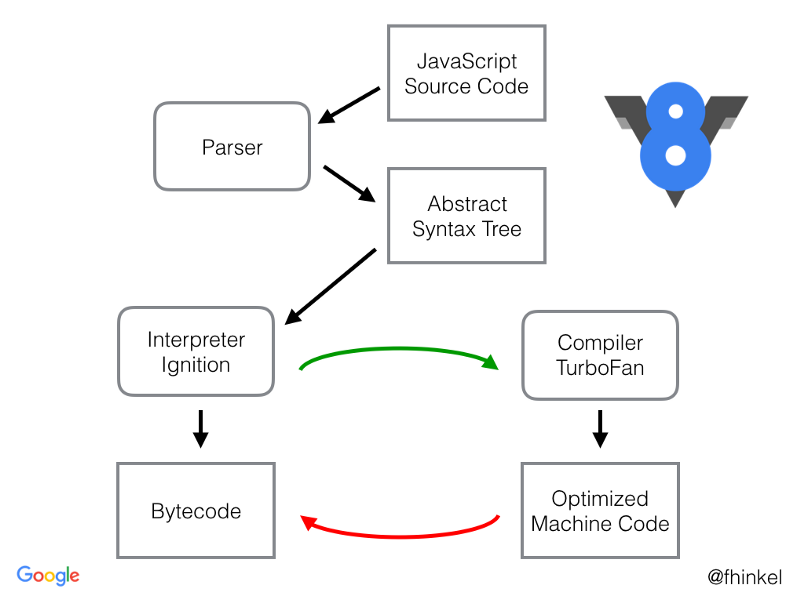
\includegraphics[width=\textwidth]{v8-architecture}
	\caption{V8 internal architecture}\label{fig:ast-v8-architecture}
\end{figure}

%TODO: add citation for the v8 internal representation

\subsection{User interface and state of the BC evaluator}\label{user-interface-and-state-of-the-bc-eval}

To keep the implementation consistent from the user perspective BC debugger should use the same user-interface as the AST. There can also be visible distinguishing between the internal state of the language~(if the language is currently inside the AST or BC evaluation mode). In the current AST implementation, there is used
\code{"debug"} as prefix printed while showing the environment browser in the debugger. This could be modified to the \code{"debugBC"} to signalize the user that the BC debugger is active.

The internal state of the GNU-R BC stack machine should be printed out to the output while the debugging. This state consists of:

\begin{itemize}
	\item Current position inside the code
	\item Stack content
\end{itemize}

Alongside the showing the current position, there would also be need to show the function bytecode. For this feature we can use the disassembler feature~\ref{implementation-of-disassembler} proposed in the first part of the analysis~\ref{analysis-of-disassembler}. Showing current position inside code can be implemented as a feature inside the disassembler but for the stack content, there has to be implemented a separate tool.

\section{Summary}

In order to improve bytecode debugging, there is a need for improving~(implementing the human-readable) disassembler. There was decided that the disassembler would be implemented as the separate \code{print.disassembly} function inside the new \code{bctools} package.

Another part of the thesis is about implementing the native bytecode debugger support into the GNU-R. The solution proposed in this thesis was inspired by the JS~V8~VM~\ref{bcdebug-implementation-in-v8} and Python~VM~\ref{bcdebug-implementation-in-python}. It consists of the implementing set of bytecode instructions~(\code{BREAKPOINT0} through \code{BREAKPOINT4}) alongside with storing of the original instructions in the separate array. This proposed solution is performance oriented because the bytecode debugger architecture should not have any negative effect on overall language performance.

Finally in the debugger, there has to be done some showing of the evaluator internal status to the user. The status consists of the bytecode of the function, current evaluated instruction, and the stack content. For showing the function bytecode and printing the current evaluator position in the code there can be reused the disassembler tool~(see~\ref{analysis-of-disassembler}) but for the dumping of the stack content, there has to be implemented completely new and separate tool.

\chapter{Realization}\label{realization}

There are three different things which have to be implemented - disassembler, stack printer and finally the BC debugger itself.

\section{Implementation of the disassembler}\label{implementation-of-disassembler}

The whole project was structured the way that \textbf{disassembler can be easily released to the CRAN repository} without the debugger. \textbf{As much as possible code is written in the R} language~(most of it in separate package \code{bctools}, but some also to the \code{compiler} one~\label{internal-parts-of-vm}) and just necessary \textbf{minimum in C} for keeping the changes into the GNU-R core code simple.

In the GNU-R language, there is the \code{compiler} package written in R. Inside it there is lying the current BC compiler and BC disassembler~(very minimal - see~\ref{current-bc-disassembler}). The changes made in order to realize the implementation of the advanced disassembler involved also modifying the \code{compiler} package. This package lies inside the GNU-R core code so the general idea about implementation was to put the just the bare minimum inside it~(the annotation of instructions~\ref{annotation-of-instructions} and putting a class into the disassembly code \ref{user-interface}). The most of the functionality was implemented then in the \code{bctools} package.

\subsection{User interface}\label{user-interface}

For better user-friendliness of the BC print function there has been made an decision to use advantage of the S3 class system~(see~\ref{R-Classes}). The old \code{disassemble} function inside the \code{compiler} package was kept intact except of the \textbf{putting class into the disasembly code}. The name of the class has been decided to be the \code{"disassembly"}. This allows us to have \textit{print.disassembly} function~(\textit{print} method of \textit{disassembly} class) inside our \code{bctools} package. That function would be then automatically dispatched once user call the \code{print} function on the object~(if the \code{bctools} package would be loaded inside user library).

The usage then changed from simple list (see figure~\ref{fig:old-disassembly-ui}) to the user friendly disassembly code~(see figure~\ref{fig:new-disassembly-ui}):

\begin{figure}[!h]
\begin{lstlisting}
#initialization
library(compiler)
f<-function(x) {
    y <- x*2
    while(x < y)
	x <- x+1

    if(x %% 2 == 0)
	x
    else
	-x
}
compiled <- cmpfun(f)

#disassembly
#  same output due internal to behavior of REPL as the
#    print(disassemble(compiled))
disassemble(compiled)

#generated output:
# list(.Code, list(8L, GETVAR.OP, 1L, LDCONST.OP,
#	2L, MUL.OP, 3L, SETVAR.OP, 4L, POP.OP, GETVAR.OP,
#	1L, GETVAR.OP, 4L, LT.OP, 5L, BRIFNOT.OP, 6L, 30L,
#	GETVAR.OP, 1L, LDCONST.OP, 7L, ADD.OP, 8L,
#	SETVAR.OP, 1L, POP.OP, GOTO.OP, 10L, LDNULL.OP,
#	POP.OP, GETBUILTIN.OP, 9L, GETVAR.OP, 1L, PUSHARG.OP,
#	PUSHCONSTARG.OP, 2L, CALLBUILTIN.OP, 10L, LDCONST.OP,
#	11L, EQ.OP, 12L, BRIFNOT.OP, 13L, 51L, GETVAR.OP,
#	1L, RETURN.OP, GETVAR.OP, 1L, UMINUS.OP, 14L,
#	RETURN.OP), list({
#   y <- x * 2
#   while (x < y) x <- x + 1
#   if (x%%2 == 0)
#       x
#   else -x
#}, x, 2, x * 2, y, x < y, while (x < y) x <- x + 1, 1, x + 1,
#   `%%`, x%%2, 0, x%%2 == 0, if (x%%2 == 0) x else -x, -x))
\end{lstlisting}
	\caption{Old disassembly user interface}\label{fig:old-disassembly-ui}
\end{figure}

\begin{figure}[!h]
\begin{lstlisting}
#initialization
library(compiler)
library(bctools) #new package
f<-function(x) {
    while(x < y) x <- x+1

	x
}
compiled <- cmpfun(f)

#disassembly
#  same output due internal to behavior of REPL as the
#    print(disassemble(compiled))
disassemble(compiled)

#generated output:
#
1:
  @ x
  GETVAR              x
  @ 10
  LDCONST             10
  @ x < 10
  LT
  @ while (x < 10) x <- x + 2
  BRIFNOT             while (x < 10) x <- x + 2	 | $2
  @ x
  GETVAR              x
  @ 2
  LDCONST             2
  @ x + 2
  ADD
  @ x <- x + 2
  SETVAR              x
  @ while (x < 10) x <- x + 2
  POP
  GOTO                $1
2:
  LDNULL
  POP
  @ x%%2
  GETBUILTIN          `%%`
  GETVAR              x
  PUSHARG
  PUSHCONSTARG        2
  CALLBUILTIN         x%%2
  @ 0
  LDCONST             0
  @ x%%2 == 0
  EQ
  @ if (x%%2 == 0) x else -x
  BRIFNOT             if (x%%2 == 0) x else -x	 | $3
  @ x
  GETVAR              x
  RETURN
3:
  GETVAR              x
  @ -x
  UMINUS
  RETURN
#
\end{lstlisting}
	\caption{Old disassembly user interface}\label{fig:new-disassembly-ui}
\end{figure}

%TODO: REDO THIS EXAMPLE

\subsection{Instruction arguments}\label{instruction-arguments}
The \textbf{BC} instruction contains the integer code identifying it followed by variable number of arguments. These arguments can be of different 5 basic types~-~-see\ref{fig:bytecode-argument-types}~(\code{BOOL}, \code{INT}, \code{LABEL}, \code{CONSTANT{\_}LABEL} and \code{CONSTANT}). The printing of the output was

The \code{CONSTANT} parameter can have two different meanings in the code. Some of the arguments could be just whole expression~(e.g. a+b+c) kept due to usage in some corner cases during evaluation~( e.g. \code{ADD} instruction is in the most cases taking the two topmost arguments. Just in some corner cases it is calling the other internal functions which are originally designed to work on the AST evaluator so they expect the expression as an input). This means that some arguments are stored because the internal implementation of the bytecode evaluator and they contains the duplicate information. The optional parameter kept due to internal purposes of evaluator was named an \code{CONSTANT{\_}DBG}.

These arguments are printed by the different functions.

\begin{figure}[H]
\begin{itemize}
	\item \code{BOOL} boolean value

	\item \code{INT} integer value

	\item \code{LABEL} - jump target / reference~(integer index) to the code array itself

	\item \code{CONSTANT{\_}LABEL} variation~(extension) of the \textit{LABEL} which allow more than one referenced index

	represented as reference~(integer index) to the constant pool where is located an array containing the references~(integer indexes) to the code array itself

	\item \code{CONSTANT} representing reference~(integer index) to the constant pool where is located constant expression~(can be either number or function)

	used for most of common cases

	\item \code{CONSTANT{\_}DBG} - constant expression inside the argument used internally just for the corner cases~(technically containing duplicitous information)
\end{itemize}
	\caption{Bytecode instruction argument types}\label{fig:bytecode-argument-types}
\end{figure}


\subsection{Annotation of instructions}\label{annotation-of-instructions}
These 6 types should be printed in different way according to the annotation. There has been created an definition for each instruction argument~(annotation of the instructions). The pretty printing disasembly function~(\code{print.disassembly} method in the \code{bctools} package) would be then taking instruction definition and printing the arguments according to the definition.

In the compiler package there is already some sort of annotation annotation specifying the number of arguments for each instruction~(\code{Opcodes.argc} list). This was list was replaced by the \code{Opcodes.descr} list containing the fully annotated instruction was named \code{Opcodes.argdescr}~(see the figure~\ref{fig:computation-of-argdescr}). To keep the old behavior the old previous \code{Opcodes.argc} list was computed from \code{Opcodes.argdescr} by applying the \code{length} function to each element~(see figure~\ref{fig:computation-of-argc}). This solution is not duplicating any information in the \code{compiler} package.

The \code{compiler} package is made with the \code{noweb} tool which is the tool to write documentation alongside with the code. Its source is written in the \textit{src/library/compiler/noweb/compiler.nw} file. Because of the fact that build command~\code{make} is not written to re-generate the source code from \code{noweb} each time the compiling is provided, we have to rerun the \code{make from-noweb} command inside the \code{compiler} to regenerate the R sources for the \code{compiler} package.

\begin{figure}[!h]
\begin{lstlisting}
<<opcode argument description>>=

SKIP.ARGTYPE<--1L
LABEL.ARGTYPE<-0L
CONSTANTS.ARGTYPE<-3L
CONSTANTS_DBG.ARGTYPE<-4L
CONSTANTS_LABEL.ARGTYPE<-5L
BOOL.ARGTYPE<-6L
INT.ARGTYPE<-7L

Opcodes.argdescr <- list(

BCMISMATCH.OP = c(),
RETURN.OP = c(),
GOTO.OP = c(LABEL.ARGTYPE),
BRIFNOT.OP = c(CONSTANTS.ARGTYPE,LABEL.ARGTYPE),
POP.OP = c(),
DUP.OP = c(),
PRINTVALUE.OP = c(),
STARTLOOPCNTXT.OP = c(BOOL.ARGTYPE, LABEL.ARGTYPE),
    #  bool is_for_loop, pc for break
.... all remaining instructions ....
)
\end{lstlisting}
	\caption{Example of instruction annotation}\label{fig:computation-of-argdescr}
\end{figure}

\begin{figure}[!h]
\begin{lstlisting}
Opcodes.argc <- lapply(Opcodes.argdescr, length)
\end{lstlisting}
	\caption{Computation of argument count in the compiler package}\label{fig:computation-of-argc}
\end{figure}

\subsection{Instruction arguments and labels}\label{instruction-arguments-labels}

Label is form of representation of the reference to the code. It is used in the jumps through the code.

\subsection{Computing of labels}

Labels are shown in the code in specific styling~(usually incrementally numbered from the 1, e.g. \code{2:}). Arguments are then referencing to these locations~(e.g. \code{{\$}2}).

There is no direct list containing locations of the labels, but it can be computed from the code. Generating of this list was done in the two-pass linear lookup through code~(see figure \ref{fig:code-generating-labels}). The result is auxiliary array containing the information direct information of number of the label~(the list is expressed as this array).

Steps to generate labels are then:
\begin{enumerate}
	\item \textbf{Initialize auxiliary array} with the size of code buffer. The each element has the default value representing, that there is no instruction which argument is pointing to that position.
	\item \textbf{Go through all instruction} in forward direction. For each argument if it contains any label~(see labels inside arguments~\ref{instruction-arguments-labels}) label then mark the according instruction on its location inside the auxiliary array.
	\item \textbf{Go through the auxiliary array} and set on each position marked as target for some instruction number of label. This number of label is calculated incrementally~(in the beginning set counter to 1, and on each marked position set the value of counter to the array and increment the counter)
\end{enumerate}

This array then would contain the information whether there is no label at the instruction~(\code{-2}) or the label~(number \code{>=0}).

\begin{figure}[!h]
\begin{lstlisting}
#first pass to mark instruction with labels
#labels is array that describes if each	Aq
#    instruction has label
n <- length(code)
#labels now contains -2=not used, -1=used
labels <- rep(-2, n)
i <- 2
instrCnt<-0 # count number of instructions
while( i <= n ) {
    v <- code[[i]]
    argdescr <- Opcodes.argdescr[[paste0(v)]]
    j <- 1
    while(j <= length(argdescr)){
        i<-i+1
        if(argdescr[[j]] == argtypes$LABEL){
            labels[[ code[[i]] + 1 ]] <- -1
        }else if(argdescr[[j]] == argtypes$CONSTANT_LABEL){
            v <- constants[[ code[[i]] + 1 ]]
            if(!is.null(v)){
                for(k in 1:length(v)){
                    labels[[v[[k]] + 1]] <- -1
                }
            }
        }
        j<-j+1
    }
    instrCnt<-instrCnt+1
    i<-i+1
}

#second pass to count labels
#loop through labels array and if
#   that instruction has label marked on it
#labels array now contains values:
#   -2=not used, -1=used, >0=index of label
i <- 2
lastlabelno <- 0;
while( i <= n ) {
    if(labels[[i]] == -1){
        lastlabelno <- lastlabelno+1
        labels[[i]] <- lastlabelno
    }
    i<-i+1
}
\end{lstlisting}
	\caption{Code for generating labels}\label{fig:code-generating-labels}
\end{figure}

\subsection{Verbosity and formatting}

Bytecode compiled function has optionally the information about location of the source. These informations are not neccesary for the evaluation of the code but are good for human-readability~(see~\ref{Exprref-and-srcref}). Alongside with this there are also some of the instruction arguments which are used just for the reason of the internal implementation and have duplicate value~(see previous~chapter~\ref{instruction-arguments}). All of these information are not necessary to be displayed for the user for the basic information but it is nice for them to provide ability to display even these information. To provide this conditional ability to show more basic or more advanced information there has been put an decision to implement more levels of the verbosity in the disassembly tool.

The levels are:

\begin{itemize}
	\item \code{0} - display only source references~(if they are available, if they aren't print expression references instead)

	see figure~\ref{fig:disassembly-verbose-0}

	\item \code{1} - the same as 0 + display bytecode version and display expression references ( if they are available )

	see figure~\ref{fig:disassembly-verbose-1}

	\item \code{2} - the same as 1 + display every operand's argument~(including ones used just for debugging)

	see figure~\ref{fig:disassembly-verbose-2}

\end{itemize}

Default value can be pre-set by \code{bcverbose} function~(provided in the \code{bctools} package).

\begin{figure}[h]
\begin{lstlisting}
1:
 - #1: function(a) while(a) a <- a-1
  GETVAR              a
  BRIFNOT             while (a) a <- a - 1	 | $2
  GETVAR              a
  LDCONST             1
  SUB
  SETVAR              a
  POP
  GOTO                $1
2:
  LDNULL
  INVISIBLE
  RETURN
\end{lstlisting}
	\caption{Disassembly output with verbose lvl 0}\label{fig:disassembly-verbose-0}
\end{figure}

\begin{figure}[h]
\begin{lstlisting}
Bytecode ver. 10

1:
 - simple_bc_verbosity1.R#4: function(a) while(a) a <- a-1
  @ a
   1: GETVAR              a
  @ while (a) a <- a - 1
   3: BRIFNOT             while (a) a <- a - 1	 | $2
  @ a
   6: GETVAR              a
  @ 1
   8: LDCONST             1
  @ a - 1
  10: SUB
  @ a <- a - 1
  12: SETVAR              a
  @ while (a) a <- a - 1
  14: POP
  15: GOTO                $1
2:
  17: LDNULL
  18: INVISIBLE
  19: RETURN
\end{lstlisting}
	\caption{Disassembly output with verbose lvl 1}\label{fig:disassembly-verbose-1}
\end{figure}

\begin{figure}[h]
\begin{lstlisting}
Bytecode ver. 10

1:
 - simple_bc_verbosity2.R#3: function(a) while(a) a<-a+1
  @ a
   1: GETVAR              a
  @ while (a) a <- a + 1
   3: BRIFNOT             while (a) a <- a + 1	 | $2
  @ a
   6: GETVAR              a
  @ 1
   8: LDCONST             1
  @ a + 1
  10: ADD                 a + 1
  @ a <- a + 1
  12: SETVAR              a
  @ while (a) a <- a + 1
  14: POP
  15: GOTO                $1
2:
  17: LDNULL
  18: INVISIBLE
  19: RETURN
\end{lstlisting}
	\caption{Disassembly output with verbose lvl 2}\label{fig:disassembly-verbose-2}
\end{figure}

%TODO: redo these examples

\subsection{Function types in the constant pool}

The constant expressions in the constant pool can of more 3 types:

\begin{itemize}
	\item regular~(ordinary) constant expressions~(e.g. numbers, array of numbers etc.)
	\item native functions~(calls to inside of the GNU R C implementation)
	\item BC compiler function code
\end{itemize}

There is no way how to print out the native functions because its structure is written and compiled inside the runtime core in C language and the R interpreter knows just the location~(function pointer) to call. These functions are printed as an \textit{$<$INTERNAL{\_}FUNCTION$>$}.

There are also stored the \textbf{BC} compiled functions which should be also printed. One way is to print out flag like \textit{$<$BYTECODE{\_}FUNCTION$>$}. The second approach is to be able to print it out nested with some indentation. The second described approach was chosen. In order to implement this feature there were introduced these 3 parameters in the disassembly tool:

\begin{itemize}
	\item \code{prefix} - the string prefix which is putted before each line printed in the whole function

	\item \code{depth} - current depthness of the recursion.

	\item \code{maxdepth} - maximal depthness for recursion~(once the \code{depth} reaches this level, the \code{$<$FUNCTION$>$} instead of calling the disassembly print would be shown in the output)
\end{itemize}

If the \code{maxdepth} would be set to the 0, the disassembly tool would print out just the \textit{$<$BYTECODE{\_}FUNCTION$>$} for every nested bytecode~(the nested BC printing would be disabled).

%TODO: add examples

\subsection{Printing functions}

%The printing of the functions were done by calling an

One type of the constant expressions in the constant array are the functions written as an expression references~(non-byte-compiled and being able to potentially evaluate with \code{eval} function). They have to be printed in user-friendly way which would not break the consistency of disassembly output. One way how to achieves that is to call the \code{dput} function printing the but it would format them line by line which is not desired output. For making the arguments look as dense as possible~(and not break consistency and compactness of the disassemble function) there has been put decision to write the function in single line. There are 2 ways how to solve this:

\begin{itemize}
	\item Write an specific call into the \textit{print.c}~(\textit{src/main/print.c}) - \textit{deparse1} function
	\item Call an \textit{dput} to print out line-by-line into the buffer by \textit{capture.output} and after that make string modifications over this output.
\end{itemize}

The first approach is more clean in order of the code but because there has been put the decision to make just minimal amount of the changes into the C core of the language~(for being able to release the disassembler in separate package) the second way was chosen.

%TODO: maybe add code example

\subsection{Printing of different types}

In the application there are different types of the actions to print~(e.g. Constants, Operators etc.). The corresponding implementation of printing functions in the disassembler is named by the dump\textit{NAME}~(e.g. \textit{dumpConstant} ) convention. The complete list of types to print:

\begin{itemize}
	\item \textbf{Constant}

		used for printing any constant value

		description of the functionality of the whole operator is described in the following chapter subsection~(see~\ref{printing-constant-expressions})

	\item \textbf{Operator}

		used for printing the operator name

		The operator names are received by the \textit{bcinfo} function from \textit{compiler} package with the \textit{.OP}~(e.g.~\textit{ADD.OP}). The knowledge that it is operator is obvious so we do not want to print it. Because of it function for printing operands is extracting the \textit{.OP} suffix and printing just the actual name~(e.g.~\textit{ADD}).

	\item \textbf{Value}

		used for printing the \textit{INT} and \textit{BOOL} argument types

		printing the expression by calling directly the \textit{cat} function

	formatting notation - directly the \textit{NUMBER}~(e.g.~1)

	\item \textbf{Label}

	formatting notation - \$\textit{LABEL{\_}NO}~(e.g.~\$1)

	\item \textbf{\code{SrcRef}} a.k.a. \textbf{source reference}

	formatting notation - \textit{SRCREF}~(e.g.~simple{\_}bc{\_}verbosity1.R{\#}4)

	\item \textbf{\code{ExprRef}} a.k.a. \textbf{expression reference}

	formatting notation - $@$\textit{EXPRESSION}~(e.g.~$@a+1$)

	the expressions are stored in the constant pool so technically they are special type of the constant expressions. For printing them we can reuse then the print function for constant ones~(the \textit{dput} and eventually even \textit{print} functions has internal support for printing out the expression references). The only difference we need to print the $@$ as prefix. So final implementation of the print function is to dump $@$ to the output and then call the function for printing out the constant expression.

\end{itemize}

%TODO: maybe add code example

\subsection{Documenting of code}

The \code{compiler} package has documentation written altogether with the code. It is managed through \code{noweb} tool~(see~\ref{annotation-of-instructions}).

The \code{bctools} package user-documentation was created with the \code{roxygen} tool~(the GNU-R inbuilt documenting system). There are several ways for developer to rebuild the documentation~(run \code{roxygen}):
\begin{itemize}
 \item \code{roxygen2::roxygenise()}, or
 \item \code{devtools::document()}, if the \code{devtools} are used, or
 \item \code{rCtrl + Shift + D}, if the \code{RStudio} is used
\end{itemize}

The second listed~(calling \code{devtools::document()}) was used during an development of this package.

\section{Implementation of the bytecode stack printer}\label{implementation-of-stack-printer}

In order to implement the BC debugger we need to be able to print the \code{BC} stack content~(see~\ref{user-interface-and-state-of-the-bc-eval}). The way how the implementation was designed was that it was written in the C language~(GNU-R language core) a printing function capable of stack of current pointer.

\subsection{Stack definition}\label{stack-definition}

Stack definition depends on the \code{TYPED{\_}STACK} typedef conditional~(see figure~\ref{fig:stack-elements-definition}). Once it is defined, the option for saved unboxed values enabled. It causes that instead of the \code{SEXP} stored in the stack every time~(which is more expensive to handle), there could be also stored raw values~(\code{int} / \code{double}). There is also \code{RAWMEM} memory which is used in the BC evaluator to store for example evaluation context frame~(but generally speaking this data type can be out of any other data type). Once the stack is enables, the stack values could be then out of these types:

\begin{itemize}
	\item \textbf{\code{int}}
	\item \textbf{\code{double}}
	\item \textbf{\code{RAWMEM}} - piece of raw memory

		its size is defined in number of \code{sizeof(SEXP)} sized  chunks
	\item \textbf{\code{SEXP}} - internal representation of the boxed object storing any value
\end{itemize}

To be able to not have to write specific code for each stack type there is implemented an macro \code{GETSTACK{\_}PTR} returning an boxed \code{SEXP} type equivalent of stack position~(no matter if the value in stack is boxed or not).

\subsection{Printing of the stack values}\label{printing-stack-values}

The printing of stack values is done through direct call of \code{deparse1} function in the C core. It is inspired by the \code{dput} function which is used for writing an \code{ASCII} representation of the R object to the text output or file. The \code{dput} function cannot be reused without any changes because it is internally evaluating the promises while dumping the output~(see~\ref{computer-promises}). However the evaluating of the promises can potentially introduce some unwanted side-effects. In order to disable the evaluating the promises the \code{deparse1} function was then called with the \code{DELAYPROMISES} argument~(instead of evaluting the promises it is showing \code{$<$promise$>$} text).

\subsection{RAWMEM stack type tag}

\begin{figure}[h!]
	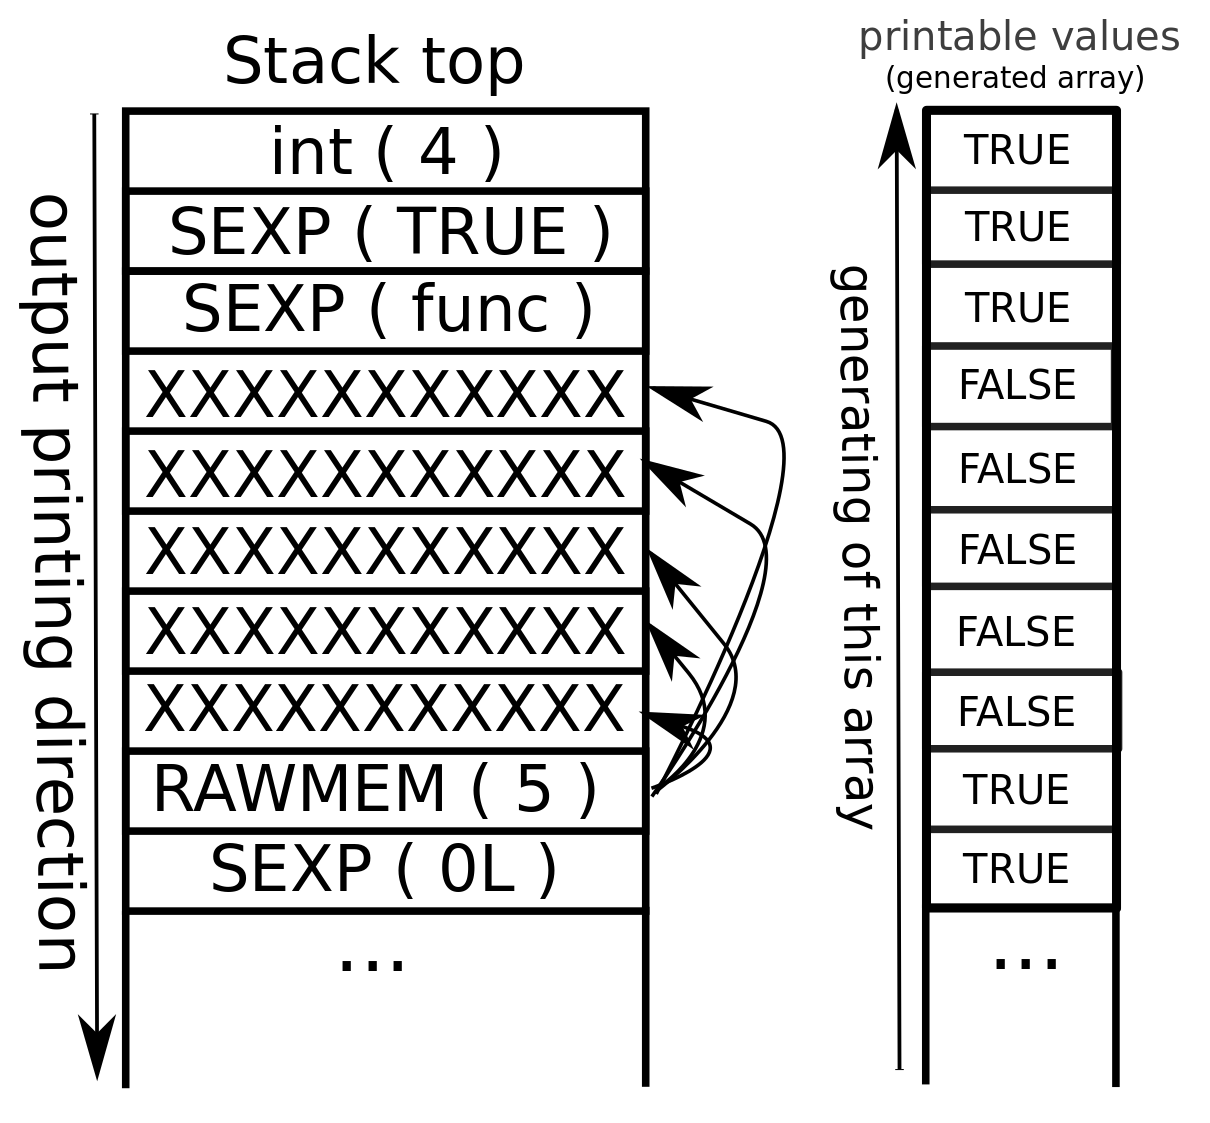
\includegraphics[width=90mm]{stack-rawmem.png}
	\caption{Definition of stack elements and generated auxiliary array showing the pritable elements}\label{fig:stack-elements-definition}
\end{figure}

In case the \code{TYPED{\_}STACK} is defined~(see~\ref{stack-definition}) then the stack values can contain raw memory chunks which cannot be printed~(see figure~\ref{fig:stack-elements-definition}). Information about size of these chunks is directed to the top of the stack. However we want to print the values in the direction from the top to the down. It results in the unsolved question whether the cell is printable or not. To be able to answer this question there has been created an auxiliary array containing the values if the cell is printable~(see figure~\ref{fig:stack-elements-definition}). It is causing some additionally complexity by running one more linear pass through the stack to fill out this array. This pass is in the forward order~(from bottom to top of the stack) so we are able to tell whether the memory is the raw or not.

The whole algorithm to dump the stack is then having two passes:

\begin{itemize}
	\item \textbf{First pass} from bottom to top to fill out the auxiliary array

			sets the \code{TRUE} value on the visited value. If the visited value is the \code{RAWMEM} type, then mark the n following~(size parameter of the \code{RAWMEM} cell) cells \code{FALSE}

	\item \textbf{Second pass} from top to bottom to actually print out the values on the stack

			works in the way that skip values for every place where the are auxiliary value is set to FALSE. If TRUE then look to the tag~(if \code{TYPED{\_}STACK} available) if is \code{RAWMEM}, then print \code{$<$rawmem of size \%d$>$} otherwise call the print function for the value~(see~\ref{printing-stack-values}).
\end{itemize}

The \code{TYPED{\_}STACK} however could also be disabled. It means that there cannot be \code{RAWMEM} stored on the stack. Even though we decided to keep the whole algorithm intact which would result in the auxiliary array having just the \code{TRUE} values~(every item is pritable). This decision would cause better maintainability of the code because there are less \code{IFDEF} compiler conditions.

\subsection{Persisting stack pointers}\label{persisting-stack-pointers}

In regards of the \textbf{BC} stack information there are currently these~(global) variables representing the current state.

\begin{itemize}
	\item \textbf{R{\_}BCNodeStackBase} - the bottom of the stack
	\item \textbf{R{\_}BCNodeStackTop} - current top of the stack
	\item \textbf{R{\_}BCNodeStackEnd} - the end of allocate space for the stack~(stack is represented internally as an array)
\end{itemize}

all of these satisfying a equation:

$R{\_}BCNodeStackBase <= R{\_}BCNodeStackTop <= R{\_}BCNodeStackEnd$


To be able to print values on the current evaluating bytecode stack we need to know when function stack frame starts and ends~(\textit{R{\_}BCNodeStackBase} points to the bottom of the whole stack and not function). There is currently not any enough information from which easily we can get an start of stack frame. To achieve this there has been added the \code{R{\_}BCNodeStackFnBase} variable representing an begin of function stack frame. It is global variable but kept and managed through context handling~(in the \textit{src/main/context.c}) to simulate the CPU function register stack frame.

\section{Implementation of the debugger}\label{implementation-of-debugger}

The main purpose of this work is enable to do the bytecode debugging. In order to do debugging we need to visualize the current bytecode internal state of the evaluating function~(debugger work in the each function separately) which consists of:

\begin{itemize}
	\item Bytecode
	\item Position inside bytecode
	\item Bytecode stack content
\end{itemize}

The position inside bytecode can be printed alongside alongside with the bytecode~(we can re-use already implemented bytecode disassembler~\ref{implementation-of-disassembler}). For the second part we already implemented the stack printer function.

\subsection{Main idea}

The main idea behind the debugger implementation is to maintain the same functionality and user interface as the current \textit{AST} implementation.

\subsection{Global design}

\begin{figure}[h]
\begin{lstlisting}
options(keep.source=TRUE)
library(compiler)
enableBCDebug(TRUE)

f<-function(a){
    c<-a+1
    d<-c+a
    c-d
}
compiled <- cmpfun(f)
debug(compiled)
compiled(2)
\end{lstlisting}
	\caption{Example of debugged function with bytecode debugger enabled}\label{fig:debugged-bcdebug-enabled}
\end{figure}

The idea used behind the debugger implementation is \textbf{inspired by the JS V8 VM}~(see~\ref{bcdebug-implementation-in-v8}). It is to replace the original instruction with special breakpoint instruction together with backuping~(saving) the original instruction alongside the bytecode. This would enable the dispatching of bytecode debug features with evaluating the same code while not causing any performance overhead in case the code is not debugged.

This feature is by default disabled. Managing the state for enabling it is done by \textit{enableBCDebug} function~(written in \textit{src/main/debug.c}) which is internally handling an \code{R{\_}is{\_}bc{\_}debug{\_}enabled} variable. See the figure~\ref{fig:debugged-bcdebug-enabled} for example.

\subsection{Instruction for debugging}\label{instruction-for-debugging}

To be able to dispatch breakpoints there has been created an specialized set of debug instructions. For dispatching breakpoint on the instruction the original instruction is replaced with it's equivalent~(according to the number of arguments) breakpoint one. The debugging instructions are:

\begin{itemize}
	\item \textbf{\code{BREAKPOINT0}}
	\item \textbf{\code{BREAKPOINT1}}
	\item \textbf{\code{BREAKPOINT2}}
	\item \textbf{\code{BREAKPOINT3}}
	\item \textbf{\code{BREAKPOINT4}}
\end{itemize}

The decision to make separate instruction for each argument count was made because of simplicity and forward compatibility. Because the normal instruction is replaced with the debug we would want to information about the number of arguments after the instruction. This would allow to have unchanged all of the functions which are iterating over the argument count instructions~(like breakpoint debugger). It is also possible that number of these function would increase in future releases of the GNU R~(by adding some feature to the BC).

%The other possible option~(which was not chosen) would have been to have just one debug instruction for whole bytecode set of instructions. This solution would save bytecode instruction space~(instead of 4 for now at least 4 instructions) and allow more simple implementation of the setting/unsetting breakpoint~(no need to look up original instruction argument count) but would add more complexity to the all functions working with the \textbf{BC} instructions argument count~(\textit{bcEncode}/\textit{bcDecode}/disassembler etc.).

\subsection{Storing of the original instruction when the breakpoint is setted}\label{storing-original-instructions}

In case the breakpoint is set~(the original instruction is overwritten by the corresponding breakpoint) we need to store the original instruction. It is necessary to keep the functionality of the evaluated BC function intact.
The idea begin implemented solution is to make an deep copy of unchanged code array to preserve the original instruction list. This copy is made the first change of the breakpoint~(first setting of the breakpoint) and attached to the \code{BCODESXP} by making new \code{CONS} cell. Once this is done we can set or unset the breakpoint on any instruction without worrying of losing any information. The setting is done by assigning the corresponding breakpoint instruction and removing is done by copying the function from the . This functionality in the \code{modifybcbreakpoint} function written in \code{C}~(the \textit{src/main/main.c} file). First passed argument is the \code{BCODESXP} object to change and the second one is the position of the instruction which has to be removed~(this position in BC code array has to have instruction and not an argument on it). The third argument is boolean flag telling whether to set or reset the breakpoint~(\code{TRUE} for setting, \code{FALSE} for removing).

The internal representation of the \code{BCODESXP} memory object holding an GNU R bytecode is the same as the \code{LISTSXP}~(the \code{BCODESXP} is internally wrapper over \code{LISTSXP}). The changes made by making an cons cell means that there is added one more nested layer. All of these functionality~(going through \code{BCODESXP} and \code{LISTSXP}) is already implemented in the Garbage Collector~(see~\ref{GC}) so there is no need to update it for support this change.

\subsection{Setting and removing debug instruction}\label{setting-and-unsetting-debug-instruction}

\begin{figure}[h]
\begin{lstlisting}
bcSetBreakpoint <- function(code, pos, is=TRUE) {
  if (typeof(code)=="closure")
    bc <- .Internal(bodyCode(code))
  else
    bc <- code
  if (typeof(bc)!="bytecode")
    stop("Internal error - code is not bytecode")

  bc <- .Internal(disassemble(bc))
  bcode <- bc[[2]]
  newbcode <- rep(bcode) #replicate original bytecode

  #loop through bytecode over instructions and find
  #   matching instruction
  setpos <- 2
  repeat{
    if(!(setpos < length(bcode) && setpos <= pos)) break
    setpos <- setpos + 1 + Opcodes.argc[[bcode[setpos]+1]]
  }

  .Internal(modifybcbreakpoint(code, setpos-1, is));

  setpos-1
}
\end{lstlisting}
	\caption{Source code of bcSetBreakpoint function}\label{fig:bcsetbreakpoint-source}
\end{figure}

To be able to set~(and unset) the debug instruction on the bytecode there has been created an \code{bcSetBreakpoint} function inside compiler package~(see fig.~\ref{fig:bcsetbreakpoint-source} for source code). It has support for both setting and removing the breakpoint on instruction~(parameter \code{is}). It is returning the position of newly set instruction which is used in the setting next breakpoint~\ref{setting-next-breakpoint}. The setted position is not usually the first of the position to set in the parameter. The reeason behind this is that this function needs to be fail-proof and cannot break the code by modifying the argument instead of the instruction~(the function is exposed to the end-user). It is internally
finding the first instruction which position~(index) is the first after the position given through \code{code} argument~(satisfies the \code{$>= code$} condition). This function is internally calling the \textit{modifybcbreakpoint} which is modifying by setting / removing the bytecode on the specified location while storing the original BC code array~(see~\ref{storing-original-instructions}).

\subsection{Listing breakpoints}\label{listing-breakpoints}

\begin{figure}[h]
\begin{lstlisting}
options(keep.source=TRUE)
library(compiler)
library(bctools)

f<-function(a){
    c<-a+1
    d<-c+ac
    c-d
}

compiled <- cmpfun(f)

#set breakpoints

 #this breakpoint would be set into position 12,
 # because at 11 is argument and
 # the implemented functionality is setting
 # the breakpoint in that cases
 # to the first following instruction
bcSetBreakpoint(compiled, 11);
 #14 is regular instruction
bcSetBreakpoint(compiled, 14);

#print the current function
# - notice the (BR) in the instruction
print(disassemble(compiled),verbose=2)

#print the bytecode instructions
# - see the 12 and 14
# -   returning an c(12,14) equivalent
print(bcListBreakpoints(compiled))
\end{lstlisting}
	\caption{Example usage of bcListBreakpoints function}\label{fig:bclistbreakpoints-example}
\end{figure}

In order to manage the breakpoint status there has been implemented a \code{bcListBreakpoints} function for listing the set ones~(it is implemented inside \code{compiler} package). This function is returning an array which contains these positions~(see figure~\ref{fig:bclistbreakpoints-example} for usage example).

%TODO: move this somewhere to end

\subsection{Setting the next breakpoint}\label{setting-next-breakpoint}

Consequential instruction does not necessary mean the following instruction right next in the bytecode array due to labels. The breakpoint for the next instruction can be either one of these:

\begin{itemize}
	\item following in the bytecode array
	\item at the position which were instruction labels pointing at~(see types of labels~\ref{instruction-arguments-labels})
\end{itemize}

To support this feature there has been developed the \code{bcSetNextBreakpoint} function~(inside the \code{compiler} package). This function is used also inside the  \code{C} code in the debugger. To support easier dispatching there it has been also written a \code{Rf{\_}breakOnNextBCInst} function which is internally dispatching an \code{bcSetNextBreakpoint} function by call to the \code{R} code through \code{eval}.

The implementation of the \code{bcSetNextBreakpoint} code is checking all possible locations for the jump locations. It is also checking if there is already set breakpoint on that position. If there is no one it is then setting there breakpoint instructions. For placing the breakpoint instruction it is using the internal call to the \code{C} function \code{modifybcbreakpoint}~(see~\ref{setting-and-unsetting-debug-instruction}).

It is also returning an array of newly added breakpoint locations. This feature is used in the implementation of the \code{BREAKPOINT} instruction~(see~\ref{implementation-of-breakpoint-instruction}) in the \code{C} core - this returned array is used to keep tracking of the added breakpoints.

\subsection{Support in the disassembly tool}\label{debugger-support-in-disassembly}

\begin{figure}[h]
\begin{lstlisting}
Bytecode ver. 10

 - #2: c<-a+1
  @ a
   1: GETVAR              a
  @ 1
   3: LDCONST             1
  @ a + 1
   5: ADD                 a + 1
  @ c <- a + 1
   7: SETVAR              c
   9: POP
 - #3: d<-c+a
  @ c
  10: GETVAR              c
  @ a
  12: (BR) GETVAR         a
  @ c + a
  14: ADD            c + a
  @ d <- c + a
  16: SETVAR              d
  18: POP
 - #4: c-d
  @ c
  19: GETVAR              c
  @ d
  21: GETVAR              d
  @ c - d
  23: SUB                 c - d
  25: RETURN
\end{lstlisting}
	\caption{Example of showing an instruction with breakpoint in the disassembly tool - (notice \code{GETVAR} instruction on position 12)}\label{fig:breakpoints-in-disassembly-example}
\end{figure}


To visualize the set breakpoints there has been added an support into the disassembly tool. The R disassembly script was modified to get 3 arrays as an bytecode input~(added field with the original code array - see~\ref{storing-original-instructions}). So the arrays now contain the constant array, code array possibly containing breakpoints and original code array which never contains any breakpoint instruction. The original array is returned every time no matter if the code array is modified or not~(in case not modified there is returned the same code array twice).

This means that we can just simply modify the disassembler to go always through the original array. Then for every instruction we would be checking in the code array~(which possibly contains breakpoints) if there is breakpoint or not. In case there is we would just simply print an mark \code{(BR)} as prefix for the instruction name to signalize that this instruction contains breakpoint~(see the figure~\ref{fig:breakpoints-in-disassembly-example} for example).

\subsection{Temporary and regular breakpoints}\label{temporary-and-regular-breakpoints}

Currently there are two types of the breakpoint inside the bytecode:

\begin{itemize}
	\item temporary breakpoint
	\item regular breakpoint
\end{itemize}

The regular ones are used for user-defined breakpoint, these ones are set by calling \code{bcSetBreakpoint} function~(from \code{compiler} package). Once the bytecode interpreter reaches them the breakpoint functionality is called and the R shows the debugger interface.

The temporary ones are used on the other hand for handling debugger commands. They are implemented with the same instruction except there are also held their locations on the bytecode local stack~(variable in which points global \code{R{\_}BCtmpBreakpoints}). This value contains an array in which each elements is representing the location of the currently set temporary breakpoint. These temporary breakpoints always point to the instruction succeeding current the evaluated one~(see~\ref{setting-next-breakpoint}).

In order to keep the garbage collector satisfied and because it is not possible to store the variable in the local protection stack~(through \code{PROTECT}/\code{UNPROTECT} function - see \ref{GC}) during \code{bcEval}, there has been dedicated one field on the bytecode stack for storing this array. The \code{R{\_}BCtmpBreakpoints} variable is then pointer~(\code{SEXP*} type) to this location. This design allows changing of this variable while modifying the bytecode body from the different evaluated context. Changing this array and not keeping an new one also reflects the fact that the modifications inside the bytecode code array are also made in-place by modifying this array.

\subsection{Implementation of the breakpoint instructions}\label{implementation-of-breakpoint-instruction}

The reason why there are implemented separate breakpoint instructions for each number of instruction arguments is its annotation. It allows us that breakpoint instruction would have the information of number of its arguments with itself. It would prevent from the breaking the bytecode code array structure. However the evaluated code inside all of the breakpoint instructions would be the same. This means that it can be simply generalized by writing single macro for all breakpoint instructions. This macro was decided to be named \code{DO{\_}BREAKPOINT} and it is containing this algorithm with the functionality for showing the debugger feature:

\begin{itemize}
	\item Remove all temporary breakpoints from the bytecode
	\item Print bytecode interpreter internal status (see~\ref{bytecode-interpreter-internal-status})
	\item Call debug browser
	\item Set \code{RDEBUG} debug flag~(see~\ref{handling-debugger-user-input})
	\item Call the original instruction~(see~\ref{threaded-and-non-threaded-design})
\end{itemize}

As you can see in the time of calling the browser there are all temporary breakpoints removed from the bytecode code array. It means that just the regular user-defined breakpoints~(see~\ref{temporary-and-regular-breakpoints}) would the printed to the output~(see~\ref{debugger-support-in-disassembly}). It is desired behavior because we do not want to print the user breakpoints which are used just for internal purposes of step-by-step feature of debugger~(see~\ref{handling-debugger-user-input}).

\subsection{Bytecode interpreter internal status}\label{bytecode-interpreter-internal-status}

Users need to know whether the interpreter is in the BC or in the AST mode. In order to achieve this the \code{"debugBC"} string was put as prefix in the each debugger browser call~(instead of \code{"debug"} in the AST evaluator).

Thing of importance while debugging the bytecode is the ability to locate the currently evaluated code~(position in code). For achieving this there has to be printed the internal status of interpreter. This was implemented in two possible ways:

\begin{itemize}
	\item \textbf{Short compact way} inspired by AST status printing
	\item \textbf{Long verbose way} showing the all information available in the \textbf{BC} interpreter - used by default
\end{itemize}

\subsubsection{The short compact way of status printing}\label{short-compact-way-of-status-printing}
It is used to simulate the AST printing behavior. It is printing the data in the same manner as AST to remain the support for the debuggers in other dependent IDEs. This way is used by default in order to keep the backward compatibility.

\subsubsection{The long verbose way showing all information}\label{long-verbose-way}
It is used for the printing the whole internal state bytecode interpreter. To support this feature there has been implemented function \code{printBCStatus()} for printing the bytecode interpreter status.

Its code is:
\begin{lstlisting}
void printBCStatus(){
    Rprintf("     --- Evaluating bytecode --- \n");
    R_printCurrentBCbody(R_BCbody, R_BCpc, TRUE, 1);
    Rprintf("     -------- Stack dump ------- \n");
    R_printCurrentBCstack(
    	R_BCNodeStackFnBase,
    	R_BCNodeStackTop);
}
\end{lstlisting}

For printing current state there is reused the calling \code{R{\_}printCurrentBCbody}~(located in \textit{src/main/eval.c}) which is internally dispatching \code{print} method of bytecode \code{disassembly} object from the \textit{bctools} package. It is called with \code{select} parameter setted to position of current evaluated instruction and \code{peephole} argument turned to \code{TRUE} to show just the surrounding area around the current instruction.

To control whether to print out the short compact way or the long way the \code{R{\_}DebugVerbose} boolean variable is used. This flag is accessible for user through the \code{debugVerbose()} function which acts like getter and setter altogether. It is returning the value of the variable as return value while having an optional parameter used for the modifying of the flag.

As you can see the code is reusing the {bytecode disassembler~(see~\ref{implementation-of-disassembler}) and stack printer~(see~\ref{implementation-of-stack-printer}).

\subsection{Debugger jumping granularity}\label{debugger-jumping-granuality}

The AST debugger is making one jump for every expression. The bytecode debugger on the other hand can jump in much more granular way~(not according to the changes of expression references but one step for each bytecode instruction). Because the short compact way should be simulation of the AST debugger it should also jump according to changes of these locations and not just by the bytecode instructions. This can be implemented by two ways:

\begin{itemize}
	\item calculate these in \code{bcSetNextBreakpoint}
	\item runtime checking
\end{itemize}

The first way is more proper in order of performance - the breakpoint would be placed on the right instruction where should be debugger functionality dispatched. The second one would work by placing the breakpoint instruction to the very next one while skipping the debugger functionality unless the change in expression reference occur~(runtime checking).

The runtime-checking was chosen due to implementation simplicity. The performance overhead would be just in case debugger is enabled which we are not worried in the first place.

On the other hand when the long verbose mode is set up. The debugger would jump directly to the following instruction which would be then visualized for user. It means that there is no need for putting any condition for skipping debug functionality on certain instructions.

\subsection{Handling of the recursive character of the bytecode}

\begin{figure}[h]
\begin{lstlisting}
/* duplicate body in case this
	function has modified */
if(BCODE_HAS_TMPBREAKPOINTS(body)){
  SEXP expr = TAG(body);
  body = CONS(
            BCODE_CODE_UNBREAKPOINT(body),
            BCODE_CONSTS(body));
  SET_TAG(body, expr);
  SET_TYPEOF(body, BCODESXP);
}

/* satisfy GC */
BCNPUSH(body); /* pushing body is neccesary
	just in case of duplicated, but pushing
	even unchanged one is easier for code
    readability */

\end{lstlisting}
	\caption{Modifying the bytecode array in the beginning of bcEval to erase breakpoints from the code}\label{fig:erase-breakpoints-in-bceval}
\end{figure}

The debugger implementation is modifying the breakpoint code while going through the code with adding an temporary breakpoints. This is done in order to support breaking on the next instruction~(see~\ref{setting-next-breakpoint}). This means that while calling recursive call there can be already set breakpoint instruction in the evaluated code. However we do not want to have any of them executed in the recursive call of the function. To solve this there was done checking~(in the beginning of \code{bcEval} function) whether the code is modified. If yes then we are creating an shallow copy of the current code without an modified byteecode code array by making new \code{BCODESXP} object created from an original code array and constant array~(see figure~\ref{fig:erase-breakpoints-in-bceval}).

Because of this implementation is allocating an new element we have to satisfy the language GC by putting its reference to the bytecode stack. It was decided to push the current evaluated body even when this change is not done. It is creating tiny memory overhead by having one unnecessary element on the stack but it is resulting in better code readability~(the value has to be also popped from the stack at the ending of evaluating).


\subsection{Threaded and non-threaded design of the application}\label{threaded-and-non-threaded-design}

Because of the speedup of the GNU-R evaluating there is support for the THREADED code. When it is on then it causes that there is no the main loop in the bytecode instruction evaluation~(see~\ref{Computed-GOTO}).

This means there were two different dispatch systems which had to be analyzed and modified to support the jumping to the different direction~(jump for calling the original instruction - inside the \textit{DO{\_}BREAKPOINT} macro).

\subsubsection{THREADED{\_}CODE defined}

\begin{figure}[h]
\begin{lstlisting}
#define NEXT() (__extension__ ({ \
    currentpc = pc; goto *(*pc++).v; \
    }))

#define BEGIN_MACHINE  NEXT();
    init: { loop: switch(which++)


#define BREAKPOINT_GOTO_ORIGIN_OP(inst) do{ \
    __extension__ ({goto *(*(inst)).v;}); \
  } while(0)
\end{lstlisting}
	\caption{Changes made for instruction handling macros in case \code{THREADED{\_}CODE} defined}\label{fig:instruction-handling-threaded}
\end{figure}

In this case the needed changes were minimal~(see figure~\ref{fig:instruction-handling-threaded}). It required adding a macro \code{BREAKPOINT{\_}GOTO{\_}ORIGIN{\_}OP} for an switching to the instruction defined in the backup array~(\code{inst} argument). Because of the implementation design of the bytecode instruction in case of the instruction operand it is holding internally position of it's label to jump to~(see~\ref{Computed-GOTO}). It is then jumping into the location defined in passed instruction value.


\subsubsection{THREADED{\_}CODE not defined}

\begin{figure}[h]
\begin{lstlisting}
#define NEXT() goto loop

#define BEGIN_MACHINE  loop: \
    currentpc = pc; \
    jmp_opcode = *pc++; \
    do_instruction: switch(jmp_opcode)

#define BREAKPOINT_GOTO_ORIGIN_OP(inst) do{ \
    jmp_opcode = *(inst); \
    goto do_instruction; \
  } while(0)
\end{lstlisting}
	\caption{Changes made for instruction handling macros in case \code{THREADED{\_}CODE} not defined}\label{fig:instruction-handling-not-threaded}
\end{figure}

In this situation things are more complicated because the whole evaluator design is one big loop. The changes in this code were described in figure~\ref{fig:instruction-handling-not-threaded}. The loop originally had  one big switch~(its beginning is defined in \code{BEGIN{\_}MACHINE} macro) which was deciding which instruction according to the value of operand~(\code{*op}). We changed this behaviour so that it is loading operand~(\code{*op}) into variable~(\code{jmp{\_}opcode}), then placed another jump label~(\code{do{\_}instruction}) and after that decided which instruction has to be evaluated according to the value of that variable~(by \code{switch} command). In the case of executing breakpoint instruction and evaluating original instruction~(through \code{BREAKPOINT{\_}GOTO{\_}ORIGIN{\_}OP}) we are setting the auxiliary variable \code{jmp{\_}opcode} to the desired instruction code. Then there is jump to the label which we added~(\code{jmp{\_}opcode}).

\subsection{Handling of the debugger user input}\label{handling-debugger-user-input}

\begin{figure}[h]
\begin{lstlisting}
...
other commands
...

}else if (!strcmp(expr, "bcstack")){
    rval = 2;
    RCNTXT* cntxt = GetBCDebugContext();
    if(R_BCIntActive)
        R_printCurrentBCstack(
            R_BCNodeStackFnBase,
            R_BCNodeStackTop);
    else
        Rprintf("Debugged context is not bytecode\n");
} else if (!strcmp(expr, "bc")) {
    rval = 2;
    RCNTXT* cntxt = GetBCDebugContext();
    if(R_BCIntActive)
        R_printCurrentBCbody(R_BCbody, R_BCpc, FALSE, 1);
    else
        Rprintf("Debugged context is not bytecode\n");
} else if () {
...
other commands
...
\end{lstlisting}
	\caption{Implemenation of \code{bcstack} and \code{bc} commands in the debugger interface}\label{fig:implementation-of-bcstack-bc-commands}
\end{figure}

The original environment browser has inbuilt support for handling and modifying the debugging~(\textit{step into}, \textit{next step}, \textit{continue} etc.) via the user input~(see~\ref{handling-debugger-user-input} implemented by setting up the \code{RDEBUG} flag and \code{R{\_}BrowserLastCommand} variable on the evaluated environment. The intent of implementing bytecode debugger interface was to reuse as much of this feature so the bytecode debugger is managed also through these variables in order to manage the debugger control. Bytecode interpreter the other hand also provides the more status information. It has been decided to extend the user interface to support showing these informations by those commands~(see implementation in figure~\ref{fig:implementation-of-bcstack-bc-commands}):

\begin{itemize}
	\item \code{bc} - print current bytecode with the position
		(internally calling \code{R{\_}printCurrentBCbody})
	\item \code{bcstack} - print current bytecode stack
		(internally calling \code{R{\_}printCurrentBCstack})
\end{itemize}

\subsection{Entry points to the bcEval functions}

While debugging bytecode there are no runtime checks inside \code{bcEval} function for the \code{RDEBUG} flag due to performance reasons. Because of this and the nature of dispatching breakpoint functionality through the special \code{BREAKPOINT} instructions~(see~\ref{instruction-for-debugging}) there is need for setting the bytecode instruction~\ref{setting-next-breakpoint} in order to dispatch bytecode functionality. This means that we have to check and pootentially apply the breakpoint instruction to the code every time the \code{RDEBUG} flag can be modified.

Currently there are two cases in which this scenario has to be handled:

\begin{itemize}
	\item At the beginning of \code{bcEval} - the bytecode function was just called
	\item Inside \code{bcEval} at the positions of the return from the function calls
\end{itemize}

The first case is handled in the beginning of the bytecode evaluation~(\code{bcEval} function). In this case there is call to the \code{Rf{\_}breakOnNextBCInst} which is setting the breakpoint to the first instruction.

The other entry point after \code{bcEval} function would be used just in case of the implementation of the conditional breakpoints~\ref{conditional-breakpoints}. If the debugger modified the state of the evaluated bytecode function~(the function was not in debug mode and now is due to calling breakpoint), add the debugging instruction to the next following instruction~(see~\ref{conditional-breakpoints}).

Because both of these cases are potentially changing the code array~(see~\ref{storing-original-instructions}) the \code{codebase} and \code{constants} array and also \code{pc} variable~(it is pointer to one of the instruction in the \code{codebase}).

\section{Simulated conditional breakpoints}\label{conditional-breakpoints}

\begin{figure}[h]
\begin{lstlisting}
SEXP attribute_hidden do_breakpoint
	(SEXP call, SEXP op, SEXP args, SEXP rho)
{
  Rboolean oldrdebug;
  oldrdebug = RDEBUG(rho);
  SET_RDEBUG(rho, 1);
  R_GlobalContext->browserfinish = 0;
  R_BrowserLastCommand = 'n';


  if(!R_is_bc_debug_enabled() && R_BCIntActive)
    warning(_("Calling breakpoint in the BC

  while bytecode debugger disabled"));

  /* Support for bytecode debugger */
  if(R_BCIntActive && !oldrdebug){
    R_RemoveBCtmpBreakpoints(
      R_BCbody, *R_BCtmpBreakpoints);
    Rf_breakOnNextBCInst(
      R_BCbody, R_BCpc, R_BCtmpBreakpoints);
  }

  return R_NilValue;
}
\end{lstlisting}
	\caption{Implementation of simulated conditional breakpoints through breakpoint() function}\label{fig:conditional-breakpoints-breakpoint}\label{simulated-conditional-breakpoints}
\end{figure}

\begin{figure}[h]
\begin{lstlisting}
#setting up the bytecode
options(keep.source=TRUE)
debugVerbose(TRUE)
enableBCDebug(TRUE)
library(compiler)

#evaluated function with breakpoint fired
# once the x variable equals to 3
f<-function(){
  for(x in 1:5){
    if(x == 3){
      breakpoint();
    }
  }
}
compiled <- cmpfun(f)
compiled()
\end{lstlisting}
	\caption{Example usage of simulated conditional breakpoints through breakpoint() function}\label{fig:example-of-conditional-breakpoints}
\end{figure}

Due to lack of the the ability of the simple and user-friendly conditional breakpoints there has been put decision to add support for simulating them. It had been done through \code{breakpoint()} function which fires the debugger functionality on the spot. It allows the user to simulate conditional breakpoint behavior by calling the environment browser as in the breakpoint instruction~(if you'd call the environment browser manually through \code{browse()} the handling of debugger through \textit{next step}, \textit{continue} etc. is not provided). The \code{breakpoint()}~(see fig. \ref{fig:example-of-conditional-breakpoints}) function is inspired by the JS \code{debugger;} command, but instead of being an separate command which would be big change in the language parser it was decided to make it a callable function.

As you can see in the figure~\ref{fig:conditional-breakpoints-breakpoint} this function is modifying the \code{RDEBUG} flag of the currently evaluating environment and resetting the temporary bytecode variables (\code{R{\_}BrowserLastCommand} and \code{browserfinish} member of function context).

\chapter{Testing and future work}\label{testing-and-future-work}

The each 3 implemented parts of this thesis were tested separately. The goal was to make as much code as possible to be able to run the automated tests on.

\section{Bytecode disassembler}

The main part of the work was done as the separate GNU-R package \code{bctools}. The R package system has it's test subsystem which runs every file in the \code{tests} directory and checks if it returns with error or not.

The test files of the \code{bctools} package include:
\begin{itemize}
	\item \textbf{basics.R} - basic functionality (printing the different cases - for loop, switch command, while loop etc.)
	\item \textbf{advanced.R} - advanced functionality
	\item \textbf{closure.R} - printing function closure
	\item \textbf{switch.R} - switch command
	\item \textbf{peephole.R} - peephole parameter
	\item \textbf{bcverbose.R} - verbose parameter
	\item \textbf{bcversion.R} - check if the current GNU R BC version is the supported one in this package~(see~\ref{R-internal-bc-representation})
\end{itemize}

Because of the simplicity the tests were not written without any testing framework. Nowadays if the test fails there is not any more detailed information where the error occurs inside the file. To support this functionality it is possible modify the tests to use \code{test{\_}that} framework which supports naming the tests and printing the name in case of it's fail.

\section{Performance testing}

%\section{Bytecode debugger}

%The \textbf{BC} debugger tests was done to make sure that there are no bugs in the code. The testing was done manually altogether with the writing of the some automated tests. Automated testing was done by step by step simulation of the step-into~(\textbf{"s" command} in the browser) by modifying beginning of the \textbf{Rf{\_}ReplIteration} function~(found in \textbf{src/main/main.c}).

%The modified function:
%\begin{lstlisting}
%int Rf_ReplIteration(
%	SEXP rho,
%	int savestack,
%	int browselevel,
%	R_ReplState *state
%  )
%{
%
%  ... variables initialization ...
%
%  if(!*state->bufp) {
%    R_Busy(0);
%    if(browselevel){
%    	/* environment browser is on */
%      strcpy((char*)state->buf, "s\n");
%    }else{
%      if (R_ReadConsole(
%      	  R_PromptString(browselevel, state->prompt_type),
%            state->buf,
%            CONSOLE_BUFFER_SIZE,
%            1)
%             == 0)
%        return(-1);
%    }
%    state->bufp = state->buf;
%  }
%
%  ... end of the function ...
%
%}
%\end{lstlisting}

%Altogether with these changes there was made an script~(modification of the test feature from the \textit{R CMD test} command) to utilize the R package test files as testing examples. The tool was comparing the output with and without an bytecode debugger support enabled and trying to simulate the same output as normal. Although this tool was not 100\% successful because internally the tests~(tested on the test directory from the \textit{bctools} package) was using catching output with it's internal feature. Running the debugger in this function meant that there was infinite recursion~(catching output which causes another catching of the output). This testing can be considered just partially successful, because it was not able to run across any of the input test cases.

%Next to this automated testing this feature was tested manually, which results were considered successful.

%\subsection{Effectiveness of testing}

%During the tests there has been observed numerous issues. Some of them were caused by the oversight during %analyzes of the \textbf{BC} compiler and/or evaluator. Example of these are:
%\begin{itemize}
%	\item handling of the \textbf{SWITCH} command arguments - lack of support for the \textbf{CONSTANT{\_}LABEL} %type - this feature support has to be also done into the disassembler code
%	\item memory issues caused by \textbf{Garbage collector} due to forgotten support for the added global %variables (such as \textbf{R{\_}BCNodeStackFnBase})
%	\item memory issue caused by modification of the body variable while duplication of the current evaluated %one~(see~\ref{setting-and-unsetting-debug-instruction}) - solved by pushing this variable onto the BC stack
%\end{itemize}

%\subsection{Side effects of the scripts}

%There are limited options to debug the memory errors inside the language \textbf{VM}~(and generally any \textbf{C} code) and finding these errors are even more difficult when the  R code is evaluated - in that case the code is internally represented as \textit{SEXP} type parameter in the \textit{eval} or eventually as an bytecode in the \textit{bcEval}.

%To be able to better understand whether some of the memory issues which occurred were caused by the injected R code and not other changes there has been made decision to rewrite some of the parts to not use \textbf{R} call to the \textbf{compiler} package but use just native \textbf{C} implementation. These parts are not having the full functionality as their \textbf{R} counterparts and were not fully tested. Although of this they can be useful for future performance improvements so they are included in the attached DVD.

%These parts of code are:
%\begin{itemize}
% \item \textbf{Rf{\_}breakOnNextBCInst}
% \item \textbf{do{\_}BCdisasm} used in \textbf{R{\_}printCurrentBCbody} function
%\end{itemize}

%\section{Conditional breakpoints}

%The conditional breakpoints are in term of the code part of the debugger support so the testing was done altogether with other testing of the bytecode debugger support.

\section{Performance testing}

TODO: performance testing

\section{Future work}

\subsection{Push into working repository}

The big part of the planned future part of the future work is to collaborate with the GNU-R core team to pushing this work into it's development and potentially even the production code. After this would be done and considering the number of people using GNU-R language~(the estimation in the 2013 was approx 2 millions), the work done in this thesis would have big worldwide effect to lot of the people.

\subsection{Merging the bctools package into the compilers}

The \code{bctools} package was developed independently as an separate disassemble feature with the minimal changes to the GNU-R VM core. This tool was also used in the debugger which is part of the VM core. When the debugger would be deployed it is suggested to merge the \code{bctools} package into the \code{compiler} while the source of the \code{bctools} one is relatively short~(approx. 600 lines). The reason why this was not already done but just proposed here as future work is that it would allow to deploy the disassembler into the working branch faster and eventually give a user-feedback for improvements before merging inside the \code{compiler} package and deploying the debugger.

\subsection{GNU R Memory optimization}

Some of the parts of the errors which were done and fixed during the development of this thesis were memory-based. During investigation of these errors there has been noticed one thing. The core of the GNU-R language is heavy dependent on the linked list memory data structure. During the modern computer implementation of the memory system this can cause a lot of memory cache misses which affect the performance. The most straightforward way to do this is to use an smallvector technique~(inspired by an llvm compiler) but the more appropriate way would be to do analysis of whole GNU-R memory subsystem optimization with focus on cache locality.

\setsecnumdepth{part}
\begin{conclusion}

The GNU-R language is one of the most popular scientific language worldwide used~(by not just scientific community). For better evaluation performance its VM internally supports the bytecode alongside with old-fashioned and slow AST interpreter. Since nowadays options for debugging the bytecode were very limited. The old disassembler showed only the raw array of instructions and constant buffer and there was no native implementation of bytecode debugging. Instead of it the evaluator was internally dispatching the AST debugger which technically resulted in code going over different code while debugging. This has changed by features proposed in this thesis.

There has been proposed and implemented changes which contains the \textbf{user friendly and easy-human readable bytecode disassembler}~\ref{implementation-of-disassembler}. The second part is about the implementation of the \textbf{native debugger support for bytecode evaluator}~\ref{implementation-of-debugger}. As the additional feature there has been added \code{breakpoint()} function which enables to add support for simulating conditional breakpoints~\ref{simulated-conditional-breakpoints}.

In the beginning of the work there is brief introduction to the problem with the motivation part~\ref{introduction}. Following is the analysis of the current implementation of the GNU-R bytecode disassembler~\ref{analysis-of-disassembler} and debugger~\ref{analysis-of-debugger} alongside with the comparison to similar tools and features in VMs of other languages. After that there are described implementation details of the work. Firstly there is described implementation of the disassembler~\ref{implementation-of-disassembler} followed by the stack printer~\ref{implementation-of-stack-printer}. Finally there is described debugger implementation~\ref{implementation-of-debugger} where is shown reuse of two previously described features. As an addition it is described the implementation of support for simulated conditional breakpoints~\ref{conditional-breakpoints}. The end of the work contains chapter about the testing of all features altogether with possible future work and improvements~\ref{testing-and-future-work}.

All the features were developed and tested and are included on the enclosed DVD. Personally it was a very good experience to work on the real language VM while implementing feature which would use millions of people. The work done in this thesis can be considered as successful.

\end{conclusion}


\bibliographystyle{iso690.bst}
\nocite{*}
\bibliography{bibliography}

%\setsecnumdepth{all}
\appendix

\chapter{Acronyms}
% \printglossaries
\begin{description}
	\item[VM] Virtual Machine
	\item[BC] Bytecode
	\item[GC] Garbage collector
	\item[AST] Abstract syntax tree
	\item[IR] Intermediate representation
	\item[JS] JavaScript
	\item[OO] Object oriented
	\item[OOP] Object oriented programming
	\item[JIT] Just in time
	\item[REPL] Read-Eval-Print-Loop
	\item[UI] User interface
	\item[ARM] Advanced RISC Machine, originally Acorn RISC Machine
	\item[CRAN] The Comprehensive R Archive Network
	\item[GCC] GNU Compiler Collection
	\item[TDD] Test driven development
\end{description}


\chapter{Contents of enclosed DVD}

%change appropriately

\begin{figure}
	\dirtree{%
		.1 readme.txt\DTcomment{instruction for the file}.
		.1 analysis\DTcomment{analysis of other implementations}.
		.1 examples\DTcomment{implementation examples directory}.
		.2 cond{\_}breakpoint\DTcomment{simulated conditional breakpoint examples directory}.
		.2 r{\_}breakpoints\DTcomment{bytecode debugger examples directory}.
		.2 r{\_}disassembly\DTcomment{bytecode disassembler examples directory}.
		.1 noncomplete{\_}functions\DTcomment{analysis of other implementations}.
		.1 bctools\DTcomment{the bctools package directory}.
		.1 r{\_}src\DTcomment{modified GNU R source}.
		.1 thesis\DTcomment{the thesis source code directory}.
		.2 DP{\_}Saska{\_}Ales{\_}2018.pdf\DTcomment{the thesis text in PDF format}.
		.2 DP{\_}Saska{\_}Ales{\_}.tex\DTcomment{the thesis text in \LaTeX{} format}.
	}
\end{figure}

\end{document}
